% Template for PLoS
% Version 1.0 January 2009
%
% To compile to pdf, run:
% latex plos.template
% bibtex plos.template
% latex plos.template
% latex plos.template
% dvipdf plos.template

\documentclass[10pt]{article}

% amsmath package, useful for mathematical formulas
\usepackage{amsmath}
% amssymb package, useful for mathematical symbols
\usepackage{amssymb}

% graphicx package, useful for including eps and pdf graphics
% include graphics with the command \includegraphics
\usepackage{graphicx}

% cite package, to clean up citations in the main text. Do not remove.
\usepackage{cite}

\usepackage{color} 

% Use doublespacing - comment out for single spacing
%\usepackage{setspace} 
%\doublespacing

% Text layout
\topmargin 0.0cm
\oddsidemargin 0.5cm
\evensidemargin 0.5cm
\textwidth 16cm 
\textheight 21cm

% Bold the 'Figure #' in the caption and separate it with a period
% Captions will be left justified
\usepackage[labelfont=bf,labelsep=period,justification=raggedright]{caption}

% Use the PLoS provided bibtex style
\bibliographystyle{plos2009}

% Remove brackets from numbering in List of References
\makeatletter
\renewcommand{\@biblabel}[1]{\quad#1.}
\makeatother


% Leave date blank
\date{}

\pagestyle{myheadings}
%% ** EDIT HERE **

%% ** EDIT HERE **
%% PLEASE INCLUDE ALL MACROS BELOW

\usepackage{psfrag}
\usepackage{subfigure}

%% END MACROS SECTION

\usepackage{todonotes}

\begin{document}

% Title must be 150 characters or less
\begin{flushleft}
{\Large
\textbf{Computable Bitstring-compressed Matrices}
}
% Insert Author names, affiliations and corresponding author email.
\\
Crysttian Arantes Paix\~{a}o$^{1\ast}$, 
Fl\'{a}vio Code\c{c}o Coelho$^{2}$, 
\\
\bf{1} Crysttian Arantes Paix\~{a}o Applied Mathematics School, Getulio Vargas Foundation, Rio de Janeiro, RJ, Brazil
\\
\bf{2} Fl\'{a}vio Code\c{c}o Coelho Applied Mathematics School, Getulio Vargas Foundation, Rio de Janeiro, RJ, Brazil
\\
$\ast$ E-mail: Corresponding crysttian.paixao@fgv.br
\end{flushleft}

% Please keep the abstract between 250 and 300 words
\section*{Abstract}
The biggest cost of
computing with large matrices in any modern computer is related to memory
latency and bandwidth. The average latency of modern RAM reads is 150 times
greater than a clock step of the processor\cite{alted2010modern}. Throughput is
a little better but still 25 times slower than the CPU can consume. The
application of bitstring compression allows for larger matrices to be moved
entirely to the cache memory of the computer, which has much better latency and
bandwidth (average latency of L1 cache is 3 to 4 clock steps). This allows for
massive performance gains as well as the ability to simulate much larger models
efficiently. In this work, we propose a methodology to compress matrices in such
a way that they retain their mathematical properties. Considerable compression
of the data is also achieved in the process Thus allowing for the computation of
much larger linear problems within the same memory constraints when compared
with the traditional representation of matrices.

% Please keep the Author Summary between 150 and 200 words
% Use first person. PLoS ONE authors please skip this step. 
% Author Summary not valid for PLoS ONE submissions.   
\section*{Author Summary}

\section*{Introduction}

Data compression is traditionally used to reduce storage resources usage and/or 
transmission costs\cite{salomon}. Compression techniques can be classified into 
lossy and lossless. Examples of lossy data compression are MP3 (audio), JPEG 
(image) and MPEG (video). In this paper, we discuss the use of lossless 
compression for numerical data structures such as numerical arrays to achieve 
compression without losing the mathematical properties of the original data.

Lossless compression methods usually exploit redundancies present in the data in 
order to find a shorter form of describing the same information content. For 
example, a dictionary-based compression, only stores the positions in which a 
given word occurs in a document, thus saving the space required to store all its 
repetitions\cite{salomon2}.  

Any kind of compression incurs some computational cost. Such costs often have to 
be paid twice since the data needs to be decompressed to be used for its 
original purpose. Sometimes computational costs are irrelevant, but the need to 
decompress for usage, can signify that the space saved with compression must be 
available when data is decompressed for usage, thus partially negating the 
advantages of compression. 

Most if not all existing lossless compression methods were developed under the 
following usage paradigm: \textit{produce} $\rightarrow$ \textit{compress} 
$\rightarrow$ \textit{store} $\rightarrow$ \textit{uncompress} $\rightarrow$ 
\textit{use}. The focus of the present work is to allow a slightly different 
usage:  \textit{produce} $\rightarrow$ \textit{compress} $\rightarrow$ 
\textit{perform mathematical manipulations} and \textit{decompress} (only for 
human reading). 

With the growth of data volumes and analytical demands, creative solutions are 
needed to efficiently store as well as consume it on demand. This issue is 
present in many areas of application, ranging from business to 
science\cite{lynch}, and is being called the \textit{Big Data} phenomenon. In 
the world of Big Data, the need to analyze data immediately after its coming 
into existence became the norm. And this analysis must take place, efficiently, 
within the confines of (RAM) memory. This kind of analyses are what is now known 
as streaming data analysis\cite{gaber2005mining}. Given a sufficiently dense 
stream of data, compression an decompression costs may become prohibitive. So 
having a way to compress data and keeping it compressed for the entire course of 
the analytical pipeline, is very desirable. 

This paper will focus solely on numerical data which for the purpose of the 
applications is organized as matrices. This is a most common data structure 
found in computational data analysis environments. The matrices compressed 
according to the methodologies proposed here should be able to undergo the same 
mathematical operations as the original uncompressed matrices, e.g. linear 
algebra manipulations. This way, the cost of compression is reduced to a single 
event of compression and no need of decompression, except when displaying the 
results for human reading. The idea of operating with compressed arrays is 
relatively new\cite{yemliha2007compiler}, and it has yet to find mainstream 
applications to the field of numerical computations. One application which 
employs a form of compression is the sparse matrix linear algebra 
algorithms\cite{dodson1991sparse}, in this case there is no alteration in the 
standard encoding of the data, but only the non-zero elements of the matrices 
are stored and operated upon. 

Larger than RAM data structures can render traditional analytical algorithms 
impracticable. Currently, the technique most commonly used when dealing with 
large matrices for numerical computations, is memory 
mapping\cite{van2011numpy,big}. In memory, mapping the matrix is allocated in a 
virtual contiguous address space which extends from memory into disk. Thus, 
larger than memory data structures can be manipulated as if they were in memory. 
This technique has a big performance penalty due to lower access speeds of disk 
when compared to RAM. 

In this paper, we present two methods for the lossless compression of 
(numerical) arrays. The methods involve the encoding of the numbers as strings 
of bits of variable length. The methods resemble the arithmetic 
coding\cite{bodden2007arithmetic} algorithm, but is cheaper to compute. We 
describe the process of compression and decompression, and study their 
efficiency under different applications. We also discuss the efficiency of the 
compression as a function of the distribution of the elements of the matrix. 
\todo{Inseri isso} Also presented are some results in relation to the 
traditional method of matrix allocation. We also consider the 
arithmetic operations to measure the efficiency of the proposed methodology.

\section*{Methods}

\subsection*{Matrix compression}

To maintain mathematical equivalence with the original data for any arithmetic 
operations, we need to maintain the structure of the matrix, ie, the ability 
to access any element given its row $i$ and column $j$ and also the numeric 
nature of its elements. In order to achieve compression, we decided to exploit 
inefficiencies in the conventional way matrices are allocated in memory. 
\todo{adicionei aqui} The analyzes presented in this article, in the first 
moment, are related to arrays of positive integers, but can be applied to 
integers and real numbers with some adaptations, which are presented in due 
course. \todo{removi isso The examples in this paper will be restricted to 
matrices with positive integer elements, but}	

The compression method is as follows. Let $M_{r \times c}$ be a matrix, in which 
$r$ is the number of rows and $c$ the number of columns. Each element of this 
matrix, called $m_{ij}$, is a positive integer. In digital computers, all 
information is stored as binary code (base 2 numbers). However, the conventional 
way to store arrays of integers is on a memory block sequence of fixed size 
(power of 2 numbers of bit), one for each element. The maximum size of a block 
is equal to the word size of the processor, which for most current CPUs is 64 
bits. Some special number such as complex number may be encoded as two blocks 
instead of one. The size of the chunk of memory allocated to each number will 
determine their maximum  size (for integers) or their precision (for 
floating-point numbers). So for matrix $M$, the total memory allocated, 
assuming chunks of 64 bits, is given by $\mathcal{B} = r \times c \times 64$.

The number of bits allocated $\mathcal{B}$, is larger than the absolute minimum 
number of bits required to represent all the elements of $M$, since smaller 
integers, when converted to base 2, require less digits. From now on, when the 
numerical base will be explicitly notated when necessary to avoid confusion 
between binary and decimal integers. 

Let's consider an extreme example: a matrix composed exclusively of 0s and 1s 
(base 10). If the matrix type is set to 64-bit integers, 63 bits will be wasted 
per element of the matrix, since the minimum number of bits needed to store such 
a matrix is $\mathfrak{b} = r \times c \times 1$. The potential economy of bits 
$\xi$ can be represented by $\xi = \mathcal{B} - \mathfrak{b} =  r \times c 
\times 63$. 

So it is evident that for any matrix whose greatest element requires less than 
64 bits (or the fixed type of the matrix) to be represented, potential memory 
savings will grow linearly with the size of the matrix.

\subsubsection*{Method 1: The Supreme Minimum (SM)}

The SM method consists in determining the value of the greatest element of 
matrix $M$, which coincides with its supremum, $max M == \sup M$  and determine 
the minimum number of bits, $b(\sup M$)(Equation \ref{eq:01}), required to store 
it. We will use capital roman letters to denote uncompressed matrices and the 
corresponding lower case letter for the compressed version.

\begin{equation} \label{eq:01}
 b(\sup M) \approx \begin{cases}
	1, &  \text{ if } \sup M \in \{0,1\} \\ 
	\lfloor \log_2(\sup M)  \rfloor + 1,  & \text{ if } \sup M > 1  
	\end{cases}
\end{equation}\todo{Será que não devemos trocar $\approx$ por = aqui? Note que 
o número de bits não é aproximado e sim o exato.}

The allocation of memory still happens in the usual way, ie, in fixed size 
64-bit chunks, only that now, in the space required for a single 64 bit integer, 
we can store for example, an entire $8\times 8$ matrix of $0_{10}$ and 
$1_{10}$. 

Let's look at a concrete example: suppose that the greatest value to be stored 
in a matrix $M$ is $\max M=1023$. Therefore, the number of bits required to 
represent it is $10$ $(1111111111)$. Let the first 8 elements of $M$ be:

\begin{equation} \label{eq:02}
  M = \begin{bmatrix}
  900 & 1023 & 721 & 256 & 1 & 10 & 700 & 20 & \hdots\\ 
  \vdots & \vdots & \vdots & \vdots & \vdots & \vdots & \vdots & \vdots & \ddots 
  \end{bmatrix}
\end{equation}

These elements of $M$, in binary, are shown in Table \ref{tab:01}. It is 
evident that the number of bits required to represent any other element must be 
lower or equal to $10$. From now on the minimum number of bits required to 
represent a base 10 integer will be refered to as its bit-length.

To store matrix $M$ it first has to be converted to base $2$ ($M_2$). Then it 
will be unraveled by column (column major, e.g. in Fortran) or by row (row 
major, e.g. in C) and its elements will be written as fixed size adjacent chunks 
of memory. The size of each chunk is determined by the type associated with the 
matrix (typically 64 bits, but always a power of 2).

According to the SM method, having determined that each element will require at 
most 10 bits, we can divide the memory block corresponding to a single 64 bit 
integer into six 10-bit chunks, which can each hold a single element of $M$. 
These 64-bit blocks will be called a bitstring. The remaining 4 bits will be 
used later. The number of bitstrings needed will be $\lfloor \frac{\dim(M) 
*b(\sup M)} {64} \rfloor +1$, where $dim(M)$ is the dimension of the matrix or 
its number of elements.

The final layout of the first 6 elements of $m$ in the first bitstring can be 
seen in \ref{eq:03}. 

\begin{equation}\label{eq:03}
 bitstring_1 = 0000\underbrace{0000001010}_{10}\underbrace{0000000001}_{1}\underbrace{0100000000}_{256}\underbrace{1011010001}_{721}\underbrace{1111111111}_{1023}\underbrace{1110000100}_{900} 
\end{equation}

Here is a step-by-step description of the application of the SM method to matrix $M$:

\begin{enumerate}
 \item Element $M_{1,1}=900 = m_{1,1} = 1110000100$ is stored in the first 
10-bit chunk of the element strip $bitstring[1]$ , which corresponds to bits 0 
to 9 (read from right to left). 
\begin{equation*}\label{eq:04}
bitstring_1 = 000000000000000000000000000000000000000000000000000000\underbrace{1110000100}_{900} 
\end{equation*}
 \item Element $M_{1,2}=1023$ is allocated in the second chunk, from bit 10 to 
bit 19. 
\begin{equation*}\label{eq:05}
 bitstring_1 = 00000000000000000000000000000000000000000000\underbrace{1111111111}_{1023}\underbrace{1110000100}_{900} 
\end{equation*}
 \item Repeat for elements $M_{1,i}$ with $i=1,\ldots,6$ which are stored on the 
remaining chunks. 
 \begin{equation*}\label{eq:06}
bitstring_1 = 0000\underbrace{0000001010}_{10}\underbrace{0000000001}_{1}\underbrace{0100000000}_{256}\underbrace{1011010001}_{721}\underbrace{1111111111}_{1023}\underbrace{1110000100}_{900} 
 \end{equation*}
 \item Element $M_{1,7}=700=1010111100$ does not fit on the remaining 4 bits of 
the first bitstring. So it will straddle two bitstrings, ie, it is divided in 
two segments $a$ and $b$, $a$ is written on the first bitstring and $b$ on the 
second.
 \begin{equation*}\label{eq:07}
  \underbrace{\underbrace{0000010100}_{20}\overbrace{101011}^{b}}_{bitstring_2}|\underbrace{\overbrace{1100}^{a}\underbrace{0000001010}_{10}\underbrace{0000000001}_{1}\hdots}_{bitstring_1}
\end{equation*}
\end{enumerate}

 Please, notice that bitstrings are written from right to left.

\begin{equation*}\label{eq:8}
  \underbrace{0000010100}_{20}\underbrace{\overbrace{101011}^a|\overbrace{1100}^{b}}_{700}\underbrace{0000001010}_{10}\ldots
\end{equation*}

Thus the compressed matrix $m = M_2$ requires less memory than the conventional 
storage of $M$ as a 64-bit integer array. An illustration of the compression 
process and the allocation of the elements of matrix M in the matrix m is shown 
in Figure \ref{fig:01}. Note that the matrix m has fewer columns that the 
matrix M, then it demands less memory to be represented. We also emphasize that 
the bits which represent the value 700 is divided in two parts and stored in 
different strips in the matrix m.

\subsubsection*{Method 2: Variable Length Blocks (VLB)}

In the SM method, there is still waste of space since for elements smaller than 
the supremum, a number of bits remain unused. 

In the VBL method, the absolute minimal number of bits are used to store each 
value. However, if we are going to divide the biststrings into variable length 
chunks, we also need to reserve some extra bits to represent the size of each 
chunk, otherwise the elements cannot be recovered once they are stored. 

Lets use again the matrix described in Equation \ref{eq:02}, where  the largest 
element is number 1023. Now instead of assigning one chunk of the bitstring to 
each element of $m$, we will assign two chunks: the first will store the number 
of bits required to store the element and the second  will store the actual 
element. The first chunk will have a fixed size, in this case, 4 bits. These 4 
bits are the required space to store the bit-length of $\sup M $, in this case, 
10.  

Lets go through VLB compression step-by-step. The largest element of $M$ is 
1023. Its bit-length is 10 which in turn is 4 bits long in base 2 (1010). Thus 
the fixed size chunk is 4 bits long for every element. 

\begin{enumerate}
 \item The first element $M_{1,1}=900$ requires 10 bits to store, so we write 
$10$ in the first chunk and $900$ in the second. 
 \begin{equation*} \label{eq:09}
 bitstring_1 = 00000000000000000000000000000000000000000000000000\underbrace{\underbrace{1110000100}_{\text{element} = 900}\underbrace{1010}_{\text{bit-length=10}}}_{M_{1,1}}
\end{equation*}
 \item Do the same for the next element, $M_{1,2}=1023$.
  \begin{equation*} \label{eq:10}
 bitstring_1 = \ldots00000000000000000000000000\underbrace{\underbrace{1111111111}_{\text{element} = 1023}\underbrace{1010}_{\text{bit-length=10}}}_{M_{1,2}}\underbrace{\underbrace{1110000100}_{\text{element} = 900}\underbrace{1010}_{\text{bit-length=10}}}_{M_{1,1}}
\end{equation*}
 \item Element $M_{1,3}=721$ is also added taking the bitstring to the state.
 \begin{equation*} \label{eq:11}
 bitstring_1 = 
 0000000000000000000000\underbrace{1011010001}_{721}\underbrace{1010}_{10}\underbrace{1111111111}_{1023}\underbrace{1010}_{10}\underbrace{1110000100}_{900}\underbrace{1010}_{10}
\end{equation*}
\end{enumerate}

So far the VLB method is more wasteful than the SM, but when we add $M_{1,4} 
=256$, we start to save some space.

\begin{enumerate}
 \item[4.] Element $M_{1,4} =256$ is added.  
 \item [5.] Elements $M_{1,5} =1$ and $M_{1,6} =10$ are added requiring a total 
of 13 bits instead of 20 with the SM method. With the addition of these elements 
we require a second bitstring. 
 \begin{align*} \label{eq:12}
 bitstring_1 &=
 \underbrace{0100}_{4}\underbrace{1}_{1}\underbrace{0001}_{1}\underbrace{100000000}_{256}\underbrace{1001}_{9}\underbrace{1011010001}_{721}\underbrace{1010}_{10}\underbrace{1111111111}_{1023}\underbrace{1010}_{10}\underbrace{1110000100}_{900}\underbrace{1010}_{10} \\
 bitstring_2 &= 000000000000000000000000000000000000000000000000000000000000\underbrace{1010}_{10}
\end{align*}
 \item [6.] The remaining two elements are added $M_{1,7} =700$ and $M_{1,8} 
=20$ in the second bit strip. 
 \begin{equation*} \label{eq:13}
 bitstring_2 = 00000000000000000000000000000000000\underbrace{10100}_{20}\underbrace{0101}_{5}\underbrace{1010111100}_{700}\underbrace{1010}_{10}\underbrace{1010}_{10}
\end{equation*}
\end{enumerate}

 We used a total of 87 bits to store matrix $m$ with the VLB method instead of 
80 bits using the SM method. However, as shall be seen later, the VLB method 
will be the most efficient for most matrices. \todo{adicionei} With the method 
VLB the resulting matrix is smaller than the original matrix.
 
\subsection*{Compression Efficiency}
 Compression efficiency depends of the data being compressed. Below, a formula 
for calculating compression efficiency is derived for both methods. They will be 
based on the following ratio: 
 
\begin{equation}\label{eq:14}
  \eta=\frac{bits\, alocated-bits\, used}{bits\,alocated}
\end{equation}
 
 Where \textit{bits alocated} above mean total bits required for standard 
storage of the matrix, without compression, while bits used mean total bits 
requires to store the matrix after compression. From now on the efficiencies are 
denoted by $\eta_1$ for the SM method and by $\eta_2$ for the VLB method.
 
\subsubsection*{SM Method}

Let $M_{r \times c}$ be the matrix we wish to compress. In comparison with a 
conventional allocation (64-bit integers), we can apply Equation \ref{eq:14} to 
calculate the efficiency of the SM method:

\begin{align}\label{eq:15}
 \eta_1 &= \frac{64 \times rc - b(max M) \times rc}{64 \times rc}\nonumber\\
 &= \frac{64  - b(max M) }{64}
\end{align}

As we see in \ref{eq:15}, $\eta_1$ does not depend on size of the matrix, only 
on the bit-length of $\max M$. If $b(\max M)=64$, $\eta_1$ is 0, ie, no 
compression is possible. On the other extreme, if the matrix is composed 
exclusively of 0s and 1s, maximal compression is achievable, 
$\eta_1=0.9843$.\todo{Alterei a proporção para 0.98, pois é o maior valor que 
pode ser obtido.}
 
\subsubsection*{VLB Method}
 
For the VLB method, compression depends on the value of each element of the 
matrix. In this method bit-lentgh variability affects the compression ratio, so 
the formula will have to include this information.

Let the $rc$ elements of the matrix $M_{r \times c}$ be divided into $g$ groups, 
each with $f_i$ numbers of bit-length $b_i = b(m_i)$. Thus $f_i$ is the 
frequency of each bit-length present in $M$. Let $k = b(b(\max M))$, ie, the 
bit length of the bit-length of $\max M$. The efficiency $\eta_2$ is shown 
below.

\begin{equation}\label{eq:16}
 \eta_2 = \frac{64 \times rc - \sum_{i=1}^{g} ( b_i + k ) \times f_i }{64 \times rc} 
\end{equation}

We can further simplify Equation \ref{eq:16} to get at shorter expression for 
the compression ratio. 

\begin{align}
 \eta_2 &= \frac{64 \times rc - \sum_{i=1}^{g} ( b_i \times f_i + k \times f_i )}{64 \times rc} \nonumber \\
  &= \frac{64 \times rc - \sum_{i=1}^{g}  b_i \times f_i  -\sum_{i=1}^{g}  k \times f_i }{64 \times rc}\nonumber \\
  &= \frac{64 \times rc - \sum_{i=1}^{g}  b_i \times f_i  - k \times\sum_{i=1}^{g}  f_i }{64 \times rc}\nonumber 
\end{align}
  
 Knowing that $$\sum_{i=1}^{g} f_i = rc, $$ we can simplify the equation above, 
obtaining (\ref{eq:17}). 
 
\begin{align}\label{eq:17}
 \eta_2 &= \frac{64 \times rc - \sum_{i=1}^{g}  b_i \times f_i  - k \times rc }{64 \times rc}\nonumber \\
  &= 1 - \frac{\sum_{i=1}^{g}  b_i \times f_i }{64 \times rc} - \frac{k}{64}
\end{align}

For this method, the highest value obtained for the data compression is 0.9687, 
when b = 1 and k = 1. However, the lower value is defined by a range of values, 
​​such that the value of $k = \frac{\sum_{i=1}^{g}  b_i \times f_i}{rc} - 64$. 
\todo{Adicionei esse trecho para ficar igual ao SM}

% Results and Discussion can be combined.
\section*{Results}

\paragraph{Random Matrix Generation.}
In both methods, compression efficiency depends on the distribution of the 
bit-lengths $b(m_{i,j})$. Thus, in this section, a method to generate a variety 
of random bit-length distributions is proposed. 

For simplicity we will model the distribution of as a mixture $X$ of two Beta 
distributions, $B_1 \sim Beta(\alpha_1,\beta_1)$ and $B_2 \sim 
Beta(\alpha_2,\beta_2)$, whose probability function is shown in Equation 
\ref{eq:18}. Since the Beta distribution is defined only in the interval $[0,1] 
\subset \mathbb{R}$ , we applied a simple transformation ($\lfloor 64 \times x 
\rfloor + 1$) to the mixture in order to map it to the interval of $[1,64] 
\subset \mathbb{Z}$. 

\begin{equation}\label{eq:18}
 f(x) =  w \, Beta(\alpha_1,\beta_1) + (1-w)\,Beta(\alpha_2,\beta_2)
\end{equation}

The intention of using this mixture was to find a simple way to represent a 
large variety of bit length distributions. The first two central moments of this 
mixture are given in \ref{eq:19} and it will be used later to summarize our 
numerical results.

\begin{align}\label{eq:19}
 E(X) &= w E(B_1) + (1-w) E(B_2) \nonumber \\
 &= w \frac{\alpha_1}{\alpha_1+\beta_1} + (1-w)\frac{\alpha_2}{\alpha_2+\beta_2}\nonumber \\
 Var(X) &= w Var(B_1) + (1-w) Var(B_2) + w (1-w) (E(B_1)^2 - E(B_2)^2)
\end{align}

In order to explore the compression efficiency of both methods, we generated 
samples from the mixture defined above, varying its parameters. From now on, 
when we mention Beta distribution we will mean the transformed version defined 
above. 

From now on, we will apply Equations \ref{eq:15} and \ref{eq:17}, to determine 
the compression efficiency of SM and VLB methods for random matrices generated 
as describe above. 

With $w=0$, a single Beta distribution is used. In Figure \ref{fig:02030405}, 
we show some distributions of bit-lengths for some combinations of $\alpha_1$ 
and $\beta_1$. From the figure it can be seen that a large variety of unimodal 
distributions can be generated in the interval $[1,64]$. 

As we are sampling from a large set distributions of bit-length, represented by 
the mixture of betas presented above, in order to make our results more general, 
we will base our analysis on the expected bit-length of a sample, since the 
efficiency of both methods depends on it. So, from Equations \ref{eq:15} and 
\ref{eq:17}, the expected efficiencies become:
 
\begin{equation}\label{eq:20}
 E(\eta_1) = 1 - \frac{k}{64}
\end{equation}

\begin{equation}\label{eq:21}
 E(\eta_2) = 1 - \frac{E(b)}{64} - \frac{k}{64}
\end{equation}

\noindent where k, in (\ref{eq:21}), is set to 7 (the bit-length required to 
represent the largest possible bit-length: 64). In (\ref{eq:20}), $k$ is the 
bit-length of the greatest element, or in the worst case, 64.

We will use the difference $D=E(\eta_1)-E(\eta_2)$ to compare the efficiency of 
the two methods. Thus a positive $D$ will favor SM method while a negative $D$ 
favors VLB method.

The expected compression efficiency in the following numeric experiments, will 
be calculated from $3$ matrices of dimension $10000$, generated as described, 
and presented in tables and figures below.
 
In Figure \ref{fig:06070809}, we can see the distribution of efficiencies and 
their difference for a sample generated from a single Beta distribution of 
bit-lengths. Note that both methods can achieve efficiencies greater than 80\% 
for matrices with very small numbers. Also note that the VLB method is more 
efficient in the majority of cases. 
 
Now let $w = 0.5$, ie, matrices will have elements with bit-lengths coming 
from a mixture of beta distributions, $B_1\sim Beta(\alpha_1,\beta_1)$ and 
$B_2\sim Beta(\alpha_2,\beta_2)$. The expected value for this mixture is shown 
in Equation \ref{eq:22}.
 
\begin{equation}\label{eq:22}
 E(B) = 0.5 E(B_1) + 0.5 E(B_2)
\end{equation}
 
For bit-lengths coming from a mixture ($w>0$), let the expected efficiencies for 
the SM and VLB methods be as given by Equations \ref{eq:23} and \ref{eq:24}. So 
now, instead of having the efficiency be a function of greatest bit-length in 
the sample (denoted as  $k$ in \ref{eq:15} and \ref{eq:17}), it will be a 
function of $max\{E(B_1),E(B_2)\}$. 

\begin{equation}\label{eq:23}
 E(\eta_1) = 1 - \frac{max\{E(B_1),E(B_2)\}}{64}
\end{equation}

\begin{equation}\label{eq:24}
 E(\eta_2) = 1 - 0.5\frac{E(B_1)}{64} - 0.5\frac{E(B_2)}{64} - \frac{max\{E(B_1),E(B_2)\}}{64}
\end{equation}
 
As before, we generate 3 matrices of dimension $10,000$ for each 
parameterization, calculate the average efficiencies (Equations \ref{eq:23} and 
\ref{eq:24}) and their difference $D$.

Before moving on to efficiency results and analyses, let's first inspect samples 
from the mixture of transformed Beta distributions. Figures \ref{fig:10111213} 
and \ref{fig:14151617}, show a few parameterizations and their resulting sample 
distributions. It is important to note that from the mixture, we can now 
generate bimodal distributions as well as the unimodal types tested before. 
Since we are making statements about efficiency as a function of the expected 
bit-length, it is important to verify if these statements hold for bimodal  
distributions as well.

After sampling uniformly ($[1,5,9,\ldots,64]$, $n=65,536$) the bit-length space 
and comparing efficiencies, we summarized the results on Table \ref{tab:02}. In 
it we see how many parameterizations (from our sample) favor each method. We can 
also look at the distribution of efficiencies on our samples for each method 
(Figure \ref{fig:1819}), which clearly demonstrate the greater expected 
efficiency of method VLB (Figure \ref{fig:19}).

As we have shown, the VLB method is more effective compressing most integer 
datasets up to 64 bits in size. This is due to its ability to exploit the 
variance in the data set and reduce the waste of bits in the representation of 
some numbers. In specific cases, where the variance in the data null or too 
small, method I will be more efficient. As a matter of fact, for matrices where 
all elements have the same bit-length, SM method  will always be better, 
regardless of bit-length (Figures \ref{fig20} and \ref{fig21}). There are only 
exception, if for bit-length 64, where neither method is able to compress the 
data. \todo{Alterei a última frase}

\section*{Discussion}

\subsection*{Calculating Efficiencies}

To determine the best compression method to apply, it's necessary to inspect the 
distribution of bit-lengths of matrix elements. When matrix elements are small 
or have nearly-constant bit-length, the SM Method is better\todo{alterei de 
best para better}, otherwise, the VLB method should be chosen.

As an example, let $M_{r\times c}$ be a integer matrix, such that the half of 
its elements have bit-length $1$ and the other half $64$. Recalling Equation 
\ref{eq:17}, now we have two groups of elements (by bit-length), $b_1=1 $, 
$b_2=64$ and $f_i = \frac{rc}{2}$ for $i = 1 \text{ and } 2$. As the greatest 
bit-length is $64$, then $k=7$. Compression efficiency $\eta_2$ can be 
calculated using Equation \ref{eq:17}. After plugging in our numbers, we obtain 
a compression of $38.29\%$.

\begin{equation*}\label{eq:25}
 \eta_2 = 1 - \frac{\sum_{i=1}^{2}  b_i \times f_i }{64 \times rc} - \frac{7}{64} 
\end{equation*}

\begin{equation*}\label{eq:26}
 \eta_2 = 1 - \frac{  1 \times \frac{rc}{2} + 64 \times \frac{rc}{2} }{64 \times rc} - \frac{7}{64} 
\end{equation*}

\begin{equation*}\label{eq:26}
 \eta_2 = 1 - \frac{  32.5  \times rc }{64 \times rc} - \frac{7}{64} 
\end{equation*}

\begin{equation*}\label{eq:27}
 \eta_2 \approx 1 - 0.5078 - 0.1093
\end{equation*}

\begin{equation*}\label{eq:28}
 \eta_2 \approx 38.29\%
\end{equation*}

The efficiency of the VLB method is influenced by the relative size of the 
bit-length groups. In this first example, we considered only two groups, each 
comprised of half the matrix elements. Let's now vary the relative frequency of 
the groups, $\frac{f_i}{rc}$, while sticking to two groups. Let's 
also \todo{Acho que tinha que tirar esse Let's also, talvez colocar Now, we are 
going to} assume that $\frac{f_i}{rc}$ is a good approximation to the 
probability of a given bit-length in a matrix, which we will denote by $p_i$.

With this definition, we can rewrite the Equation \ref{eq:17}, which becomes 
\ref{eq:29}. In Equation \ref{eq:29}, the $\frac{f_i}{rc}$ is replaced by $p_i$, 
representing the probability of elements from group $i$ in matrix M.

\begin{equation}\label{eq:29}
 \eta_2 = 1 - \frac{\sum_{i=1}^{g}  b_i \times p_i }{64} - \frac{k}{64} 
\end{equation}

\noindent with

\begin{equation}\label{eq:30}
 p_i = \frac{f_i}{rc}
\end{equation}

With the Equation \ref{eq:29} can analyze the influence of bit-length 
probability in compression efficiency. In this example, $p_1$ and $p_2$ 
represent the probability of elements of bit-lengths 1 and 64, respectively. 
Thus, efficiency is defined in Equation \ref{eq:31}. 

\begin{equation}\label{eq:31}
 \eta_2 = 1 - \frac{1 \times p_1  + 64 \times p_2}{64} - \frac{7}{64} 
\end{equation}

Now, we can determine which probabilities give us the best and worst compression 
levels. When $\eta_2=1$, then the efficiency is maximal and if $\eta_2=0$, a 
efficiency is minimal. To calculate the values ​​of $p_1$ and $p_2$ for both 
extreme values of $\eta_2$,  we must solve the linear systems shown in Equations 
\ref{eq:32} and \ref{eq:33}. The first equation on both systems come from the 
law of total probability. The second comes from \ref{eq:31} after setting 
$\eta_2$ to $1$ and $0$, respectively. 

\begin{equation}\label{eq:32}
  \eta_2 = 1 :\left
  \{\begin{matrix}
    p_1 + p_2 = 1\\ 
    p_1+64p_2 = 7
  \end{matrix}
  \right.
\end{equation}

Solving the system above, we find that  when $p_1=0.9047$ and $p_2=0.0953$, 
efficiency is maximal, and in this particular case is equal to 87.5\%.

\begin{equation}\label{eq:33}
  \eta_2 = 0 :\left
  \{\begin{matrix}
    p_1 + p_2 = 1\\ 
    p_1+64p_2 = 57
  \end{matrix}
  \right.
\end{equation}

Thus, when $p_1=0.1111$ and $p_2=0.8889$ the efficiency is minimal for the VLB 
method. For other combinations see Table \ref{tab:03}. Looking at this table, 
one can see two negative efficiencies, when ($p_1$,$p_2$) assume the values 
​​(0,1) and (0.1,0.9). This correspond th cases, when the method increases, the 
memory requirements instead of decreasing it.


So far, we have examined only two groups (hence two probabilities) of bit-length 
for the sake of simplicity. Before, we generalize to probability distributions 
let's take a quick look at the efficiencies for more groups, with uniform 
probability:

\begin{itemize}
  \item 3 groups with bit-lengths 1, 32 and 64 bits, efficiency $\eta_2=0.3854$,
  \item 5 groups with bit-lengths 1, 16, 32, 48 and 64 bits, efficiency $\eta_2=0.3875$,
  \item 8 groups with bit-lengths 1, 8, 16, 24, 32, 40, 48, 56 and 64 bits, efficiency $\eta_2=0.3888$
\end{itemize}

When the distribution of the group probabilities is uniform, ie, the groups 
have approximately the same size, efficiency is basically the same, regardless 
of the number of groups.

Now, we can leverage the notion of bit-length probabilities, and study 
efficiency when bit-lengths follow some commonly used discrete probability 
distributions: Discrete Uniform, Binomial and Poisson. For all the experiments, 
we assume $k=7$, that is, the maximum possible bit-length is 64 bits. Thus, 
efficiency obtained will not be the best possible, since for that we would need 
assume small values of $k$ (Equation \ref{eq:29}). 

\subsection*{Discrete Uniform}
Let the bit-lengths of the matrices be distribute according to the Uniform 
distribution $U(a=1,b=64)$, which means bit-lengths may take values in the set 
$\{1, 2, 3, $\ldots$, 64\}$ with equal probability, ie, $\frac{1}{64}$. 

\paragraph{Theoretical Efficiency:}
Let the random variable $B \sim U(a=1,b=64)$ represent the  bit-length of the 
elements of matrix $M$. Then $E(b_i) = \sum_{i} b_i \times p(b_i) = 
\frac{a+b}{2}$.  Applying this result to the expected compression efficiency of 
VLB method (Equation \ref{eq:29}), we have

\begin{equation}\label{eq:44}
 E(\eta_2) = 1 - \frac{E(B)}{64} - \frac{k}{64} 
\end{equation}

\noindent assuming all bit-lengths are possible, i.e., $a=1$ and $b=64$, and 
hence $k=7$, we can calculate $\eta_2$: 

\begin{equation}\label{eq:45}
 E(\eta_2) = 1 - \frac{\frac{1+64}{2}}{64} - \frac{7}{64} \approx 38.28\% 
\end{equation}

This result agrees with the numerical estimates presented in Table \ref{tab:04}.

\paragraph{Numerical Estimates:}

To calculate the VLB efficiency, we generated a matrices with 100 ($M_{10 \times 
10}$), 10,000 ($M_{100 \times 100}$) and 1,000,000 ($M_{1,000 \times 1,000}$) 
elements with 1, 8, 16, 32 and 64 number of bits.  The average efficiency (Table 
\ref{tab:03}) is calculated from a 1,000 replicates of each matrix size. As 
expected the compression efficiency gets better with lower expected bit-length.

\subsection*{Binomial Distribution}

For the binomial distribution, we will use $Bin(n, p)$, with the number of 
trials $n$ representing the greatest possible bit-length in the matrix, and $np$ 
giving us the expected bit-length. 

\paragraph{Theoretical Efficiency:}
Let bit-length $(B)$ be a random variable with Binomial distribution, $B \sim 
B(n=64,p=0.5)$, $E(b_i) = \sum_{i} b_i \times p(b_i) = n \times p$ and the 
efficiency becomes (with $k=7$):

\begin{align}\label{eq:47}
 E(\eta_2) &= 1 - \frac{64 \times p }{64} - \frac{k}{64}  \\
  &= 1 - \frac{64 \times 0.5 }{64} - \frac{7}{64} \approx 39.05\% \nonumber
\end{align}

Which again agrees with estimates in Table \ref{tab:05}.

\paragraph{Numerical Estimates:}

For these experiments, the parameter n represents the maximum bit-length of 
matrix elements and takes values in $\{1, 8, 16, 32, 64\}$. In this case, we 
evaluate the efficiency as a function of the parameter $n$, and matrix size. 
Even though efficiency does not depend on matrix size, we tried different sizes 
to test the stability of the compression algorithm. Results are shown in Table 
\ref{tab:05}. As expected, smaller bit-lengths lead to higher compression 
efficiencies. 

\subsection*{Poisson Distribution}
With bit-length derived from a Poisson($\lambda$), the parameter $\lambda$ 
corresponds to the expected bit-length. For the purpose of this analysis this 
Poisson distribution is truncated at 64.

\paragraph{Theoretical Efficiency:}
Let bit-length $B \sim Poisson(\lambda=32)$. In this case, $E(b_i) = \lambda$, 
with $k=7$,  the efficiency becomes: 

\begin{align}
 E(\eta_2) &= 1 - \frac{\lambda}{64} - \frac{k}{64} \label{eq:49} \\
 &= 1 - \frac{32}{64} - \frac{7}{64} \approx 39.06\% \label{eq:50}
\end{align}

This result is in accordance to Table \ref{tab:06}.

\paragraph{Numerical Estimates:}
The results for this simulation can be seen in \ref{tab:06}. Note that 
increasing the number of bits to represent numbers increases, there is a loss of 
efficiency in the compression process. In this case, we did not simulate for 
$\lambda=64$ since a large portion of the samples would fall above the maximum 
bit-length, but \todo{coloquei ", but", aqui} we are considering for this 
analysis. 

These results show that a good compression is guaranteed when bit-lengths are 
distributed according to the tested distributions regardless of sample size. 


\section*{Library Implementation }

The methodology employed in this this paper includes the SM method, which was implemented in a library for Fortran. The 
overloaded operations were assignment, addition, subtraction, multiplication, transpose, and maximum of a matrix. 
Although only few significant operations of matrices presented ovearload, any other operation can be performed, since 
the methods for inserting and collecting an element in a matrix of bitstring were implemented. With these two methods, 
as long as they are properly adapted into algorithms, it becomes possible to implement any other desired operation.

The method was also extended to allow for the allocation of real and integer numbers, besides positive integers, inside 
the matrix bistring. Some adjustments were made so that the other groups of numbers could be represented. In order to 
represent the integers with signs, it is necessary to use two's complement, as it is applied to thein accordance to 
traditional methods.

The SM method uses a range of bits to store the values in such a way that
the size or number of bits used is important to represent the highest value in the bitstring matrix. The adaptation 
consists in determining the largest value to be stored considering the absolute value of the number. That done,
when the number is negative, it is necessary to rewrite it since, due to the sign, this will be written in the form of 
two's complement. The purpose of this conversion is to optimize library processing. Take the following as an example: 
the number 5, when represented in a 32-bit integer, is defined as:

\begin{equation}\nonumber
 5 = 00000000 00000000 00000000 00000101
\end{equation}

However, if the number is negative, this is represented in the form of two's complement. Therefore, the number -5 is 
represented as:

\begin{equation}\nonumber
 -5 = 11111111 11111111 11111111 11111011
\end{equation}

Note that the bit positioned more to the left should be used to inform that the number is -5. For the purpose of 
optimization of the library, it was chosen to conversion of positive numbers to negative numbers and use of 1 
bit to represent the sign. (Dúvidas aqui)

In turn, in order to represent real numbers, a conversion procedure of real numbers to integer numbers was used. The 
real number is multiplied by a power of ten and is then immediately truncated. The real numbers in a binary system of 64 
bits are represented using a bit to represent the sign of the number, 11 bits to the exponent, and 52 bits to the 
mantissa. Note that 1 bit is still used implicitly, according to the IEEE-754 standard. In summary, the mantissa is 
represented in the base $2^{-1}$, $2^{-2}$, $2^{-3}$, $\hdots$, $2^{-52}$. Depending on the value to be represented, 
loss of information can take place, which is related to the accuracy of the type used. In this case, considering a real 
number with double precision, the demand of 64 bits to represent each one occurs, and in some cases, the number to be 
represented is an approximation. As an example, consider that the number to be stored is 1.109. Following the 
traditional system, the number 1,109 is represented by

\begin{equation}\nonumber
  0011111111110001101111100111011011001000101101000011100101011000
\end{equation}

We consider that the power used is $10^3$, that is, the number which needs to be stored would be 1109. In binary, that 
number is represented by 10001010101. Note that the number of bits required is smaller, but depending on numerical 
accuracy, the compression methods suggested are ineffective. When the power of 10 is used, it must be applied across the 
matrix. This conversion allows the proposed methods to be applied to a set of real numbers. It should be taken into 
account that the greater the power of 10 used, which is associated with the conversion of the real number, the larger 
the set of bits will be required to represent the converted number. This affects the efficiency of data compression. The 
use of the library to represent real numbers is conditioned to a study of the necessary level of precision to solve the 
problem.


\section*{Library Application}

In order to create an application, some elementary matrix operations. Different operations have been performed by 
measuring the execution time of each. We basically, considered the attribution of a constant to all the elements of a 
matrix; the addition, subtraction and multiplication of the elements of a matrix by a constant, the addition, 
subtraction and multiplication of matrices. In addition to that, the calculation of  the transposed matrix and the 
maximum an array were also considered. This measure was used to evaluate the efficiency of the method implemented when 
compared to traditional methods.

One of the characteristics of bitstring matrices is that the operations per column, in the case of implementation in 
Fortran, can be parallelized. This reduces the execution time, compared to traditional methods. Therefore, in order to 
achieve this optimization, threads implementations were used for the implemented operations.

As a test methodology, all the described operations were also compared to traditional methods. The matrix dimensions n x 
n used were $n = 10$, $100$, $1,000$, $10,000$, $20,000$ to $100,000$, by $10,000$. We emphasize that the matrix,  
created with a 1,000 dimension has $10^6$ elements, while the one with a 100,000 dimension has $1 \times 10^{10}$ 
elements. With the increase of the size of the matrices, a larger amount of memory must be reserved to allocate the 
numbers. The compression effect of the matrices can be verified in the results since by the proposed method the matrix 
is ​​directly loaded into the main memory, avoiding the need for access to the secondary memory.

XXXXXXXXX

Another library application was the implementation of the algorithm in order to deal with the problem of arrays of 
collaborative filtering \cite{cf}. These arrays have large dimensions due to the number of users and products. Each 
element of this matrix stores the rating of a user with respect to a specific product. With this information, it is 
possible to specify a product for a determined customer.

The manipulation of these matrices, depending on the amount of memory to be allocated, are one of the possible 
applications of the methods proposed in this work, since it promotes the compression and data allocation in the main 
memory. The allocation of the matrix within the main memory makes the access time to the elements much smaller than when 
the matrix is stored in secondary memory. This latter type of storage is used in some already mentioned techniques. As 
an example, let us examine the manipulation of a CF matrix, evaluating the access time to the elements and especially 
the size of the memory required to run such operation. The algorithms applied to this matrix were the average per-use 
and the bias from mean \cite{cf}, this last one of the simplest algorithms for predicting the rate of users.

An example of the application of the methodology presented is shown in Figure \ref{fig22}. In this figure, the matrix 
with normal and bitstring formats are displayed. In both matrices, the information is represented and can be accessed. 
Therefore, it becomes possible to apply the selected algorithms.

yyyyyyyyyyyyyy

\section*{Conclusion}

In this paper, we have focused in the compression of matrix data, since this is
one of the most important application the authors foresee. However, the
compression methodology presented can be applied to any numerical data
structure, with gains to performance and memory footprint\cite{teseCrysttian}. 

Further discussions about doing computation with such compressed data-structures
will be the subject of another manuscript (in preparation) in which we will
present details about the implementation of the compression algorithm, and
benchmarks on classical linear algebra tasks such as those in
Linpack\cite{dongarra1979linpack}.

For the compression calculations presented in this paper we limited bit-lenght of integers to 64 bits. However the 
compression would work in the same way as discussed for computer architectures with larger word sizes. 

Representation of floating point numbers is also possible within the proposed compression framework, but at the expense 
of precision in their representation. Although this may sound like a limitation, when we take into consideration that 
most experimental data have fewer ``significant'' digits than the maximal precision available in modern computers, 
fairly good compression may still be achievable for floats. 

% You may title this section "Methods" or "Models". 
% "Models" is not a valid title for PLoS ONE authors. However, PLoS ONE
% authors may use "Analysis" 


% Do NOT remove this, even if you are not including acknowledgments
\section*{Acknowledgments}
We would like to thank Claudia Torres Code\c{c}o, Moacyr Silva and Paulo
Cezar Carvalho for fruitful discussions and key ideas which helped improve the
manuscript.

%\section*{References}
% The bibtex filename
\bibliography{plos.bib}

\section*{Figure Legends}

\begin{figure}[h]
  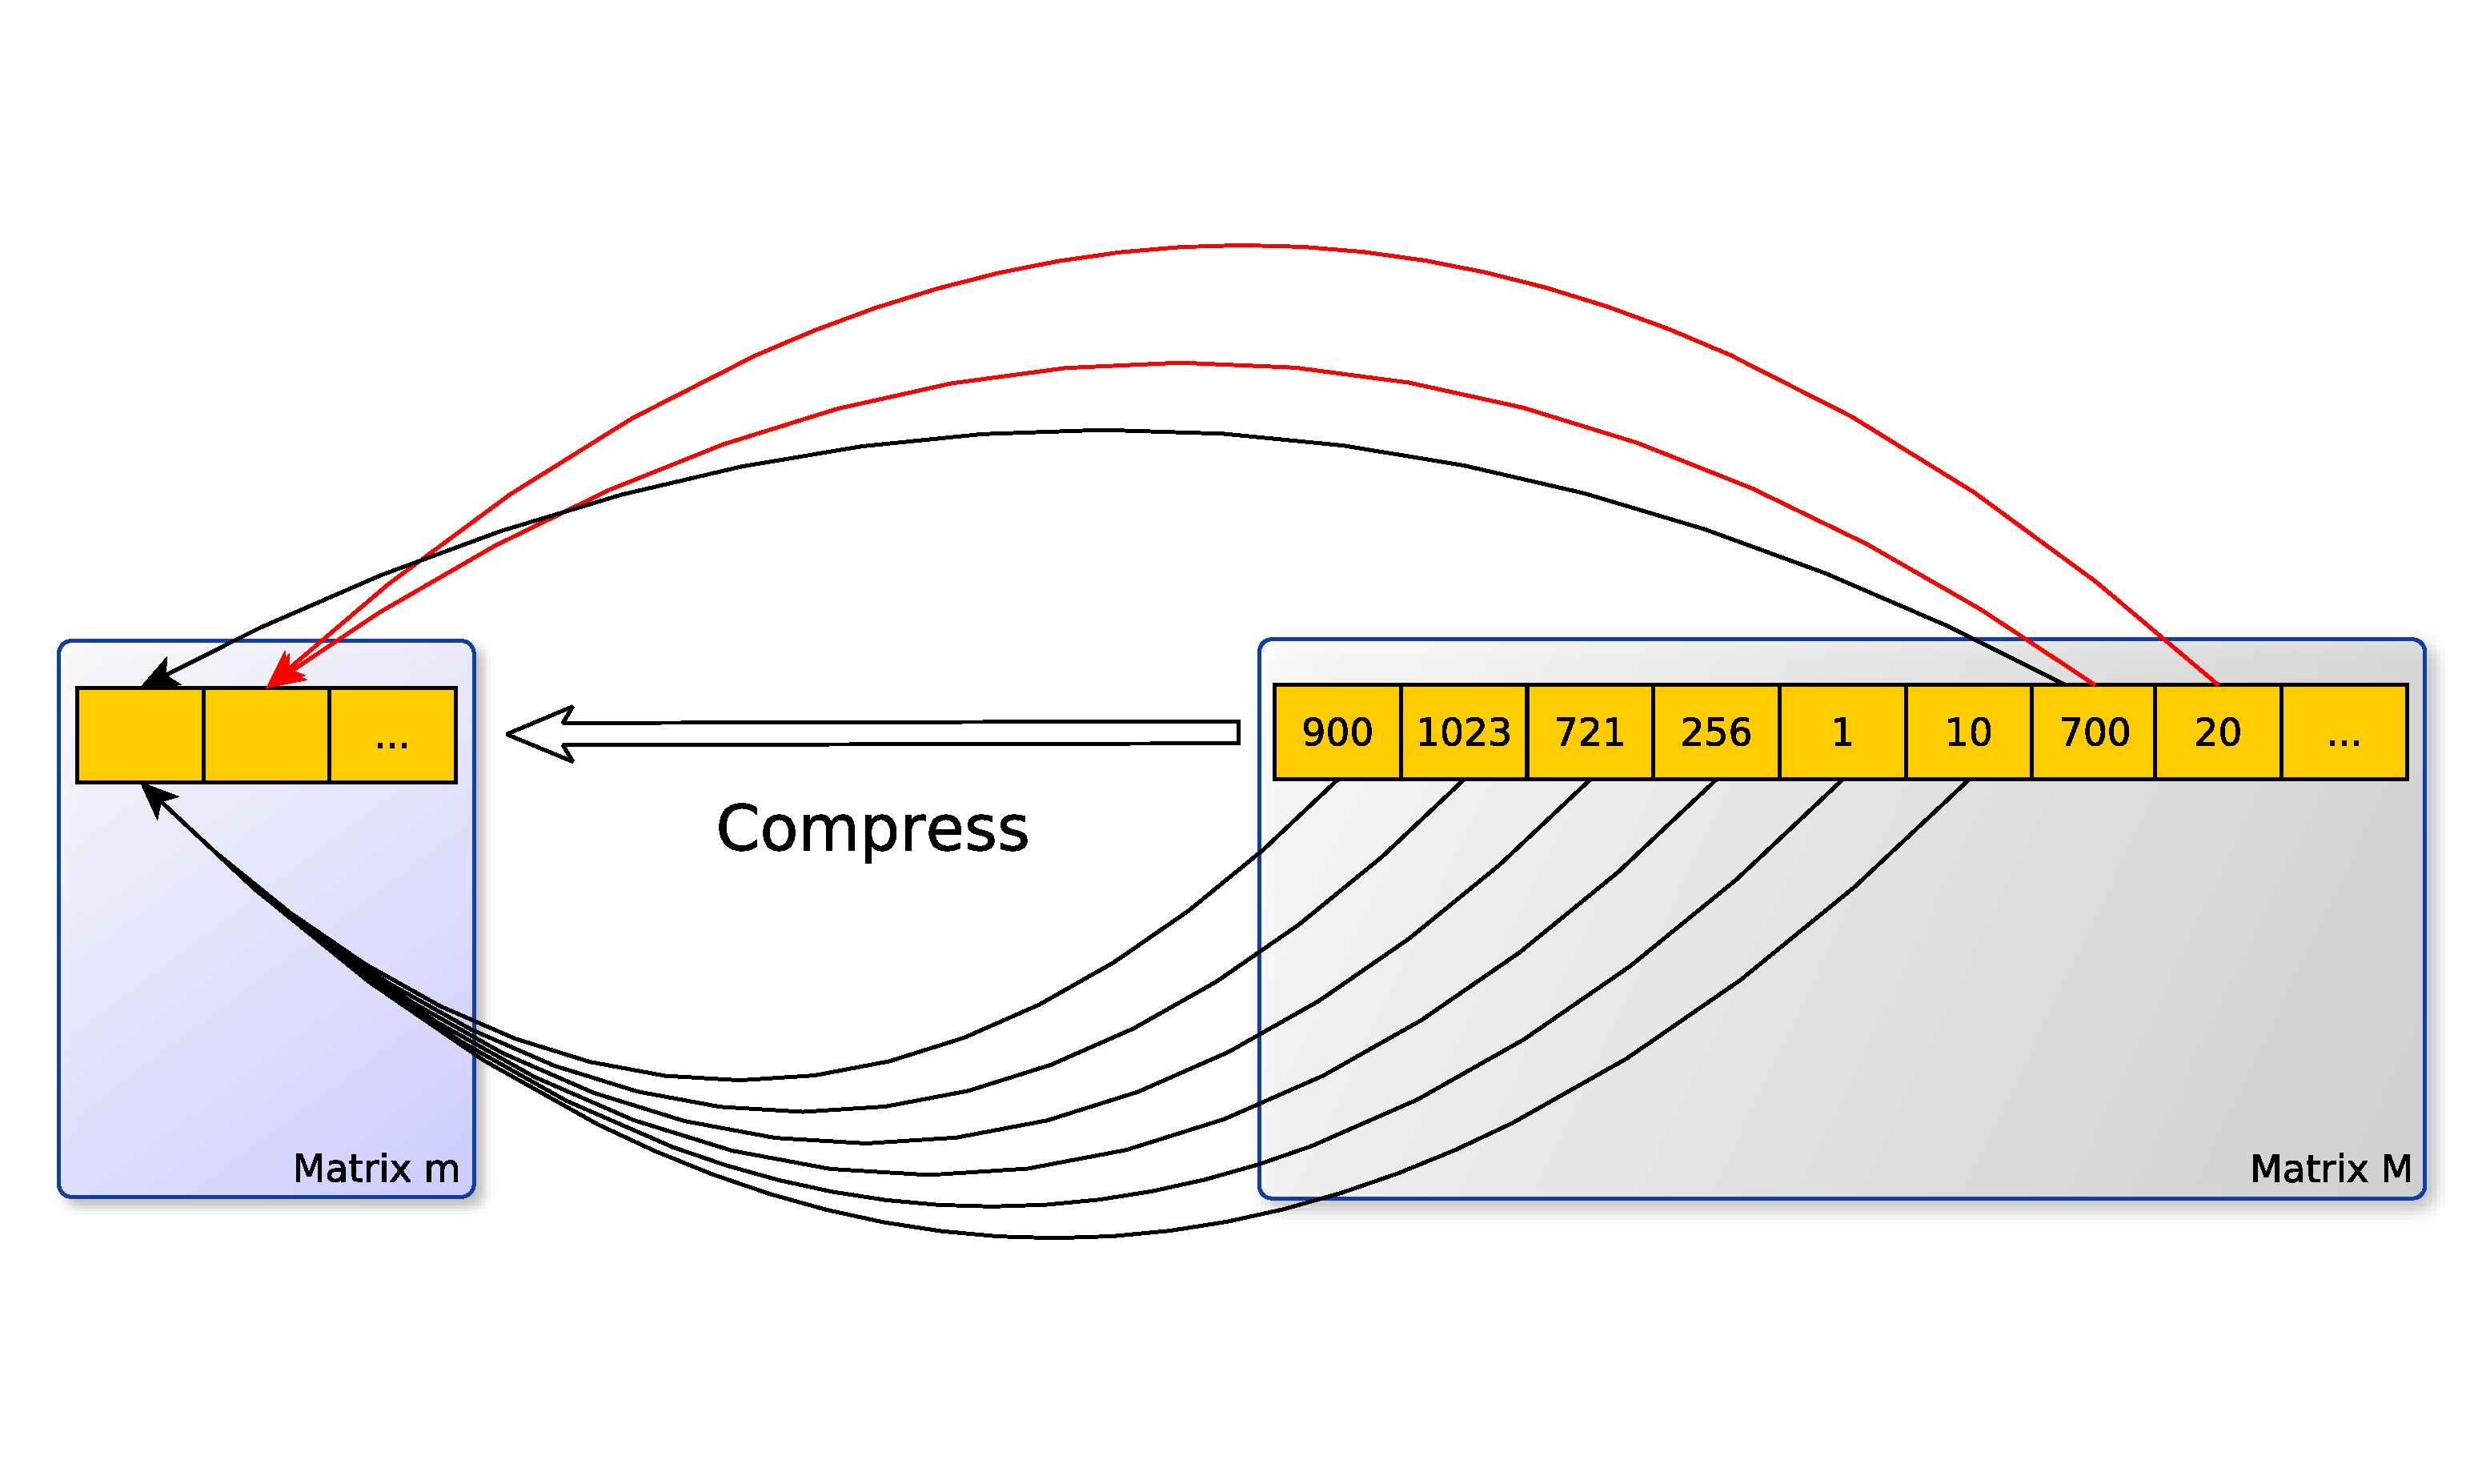
\includegraphics[scale=0.3,clip]{fig01}
  \caption{Representation of the compression process and allocation of 
elements of matrix M in the matrix m. The strip of value 700 is divided in two 
parts and stores in different strips in the matrix m.}
  \label{fig:01}
\end{figure}

\begin{figure}[h]
  \centering
  \subfigure[$\alpha=1,\beta_1=1$]{
   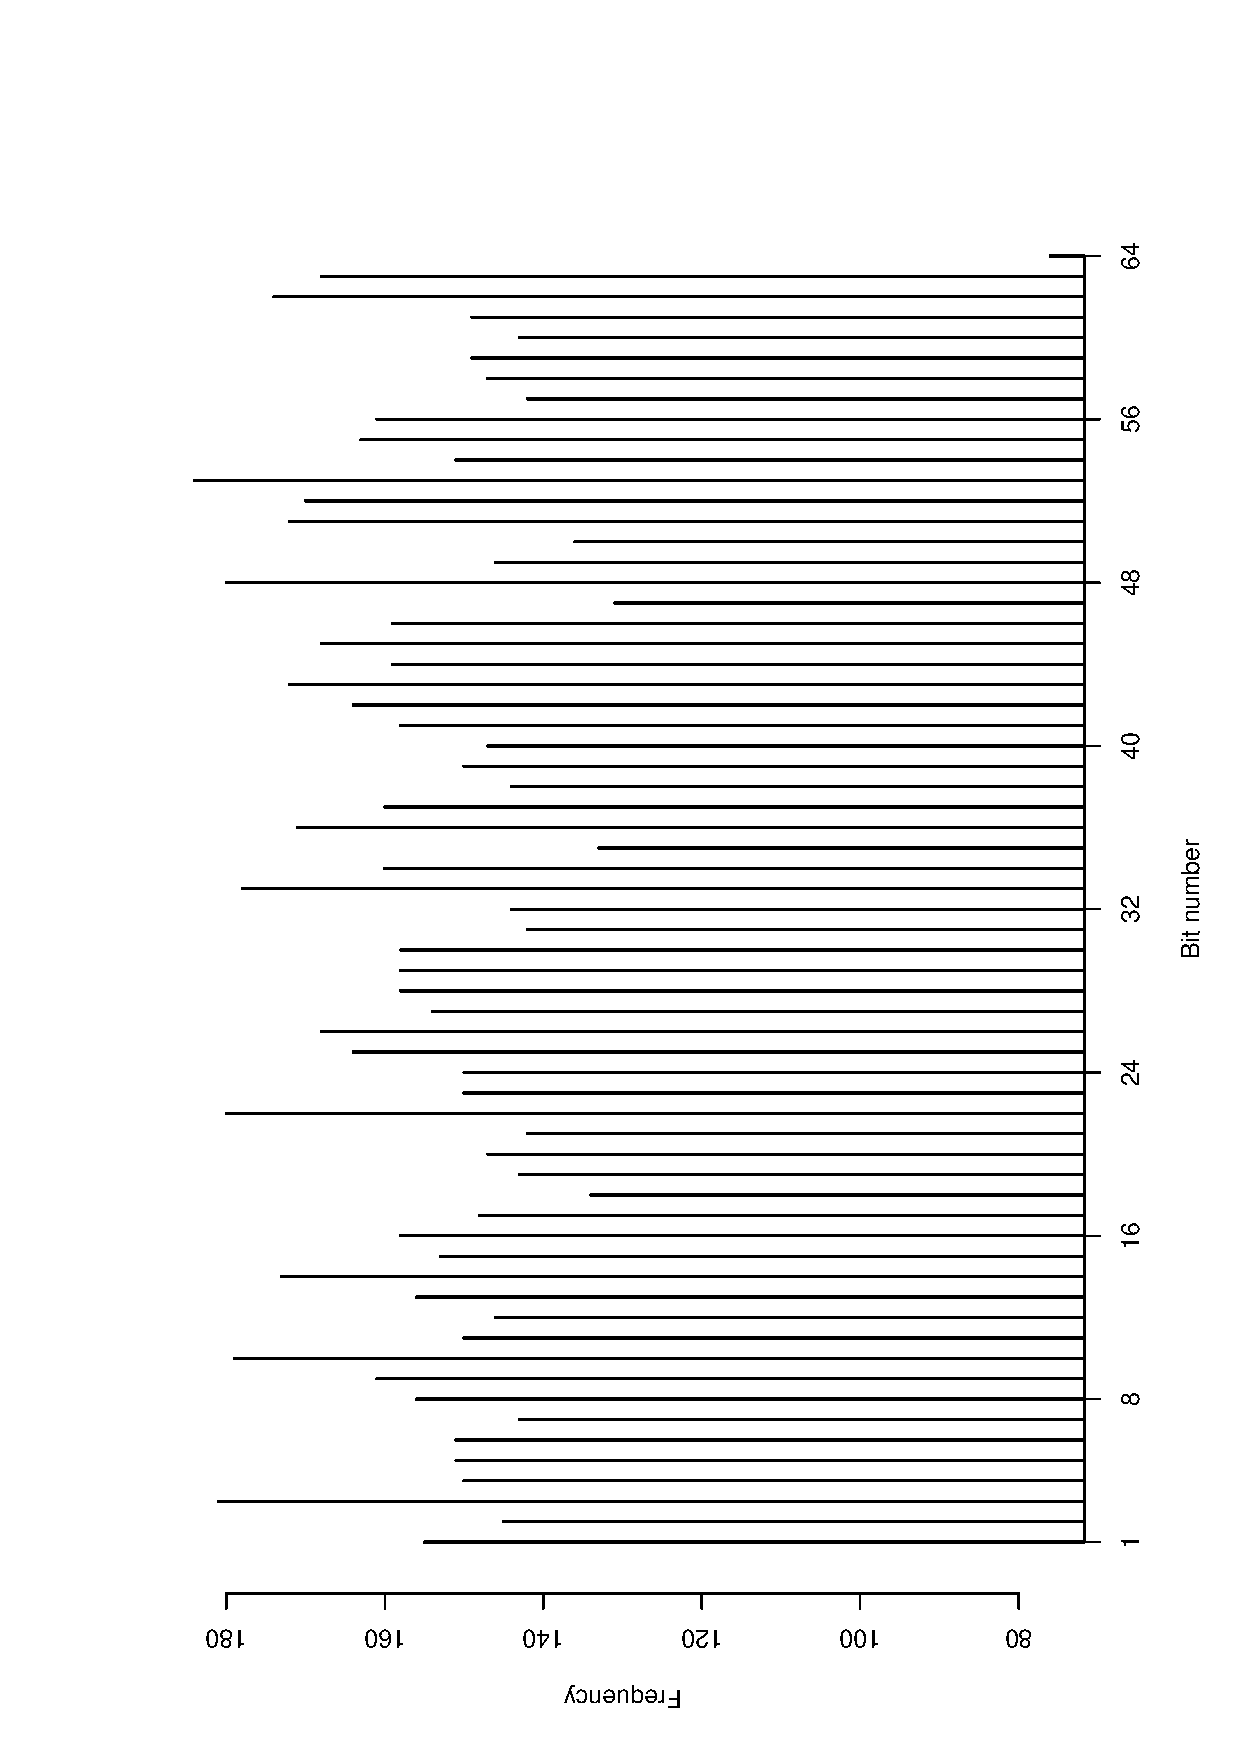
\includegraphics[scale=0.25,angle=-90,clip]{fig02}
  }
  \subfigure[$\alpha=1,\beta=32$]{
   \includegraphics[scale=0.25,angle=-90,clip]{fig03}
  }
  \subfigure[$\alpha=32,\beta=1$]{
   \includegraphics[scale=0.25,angle=-90,clip]{fig04}
  }
  \subfigure[$\alpha=64,\beta=64$]{
   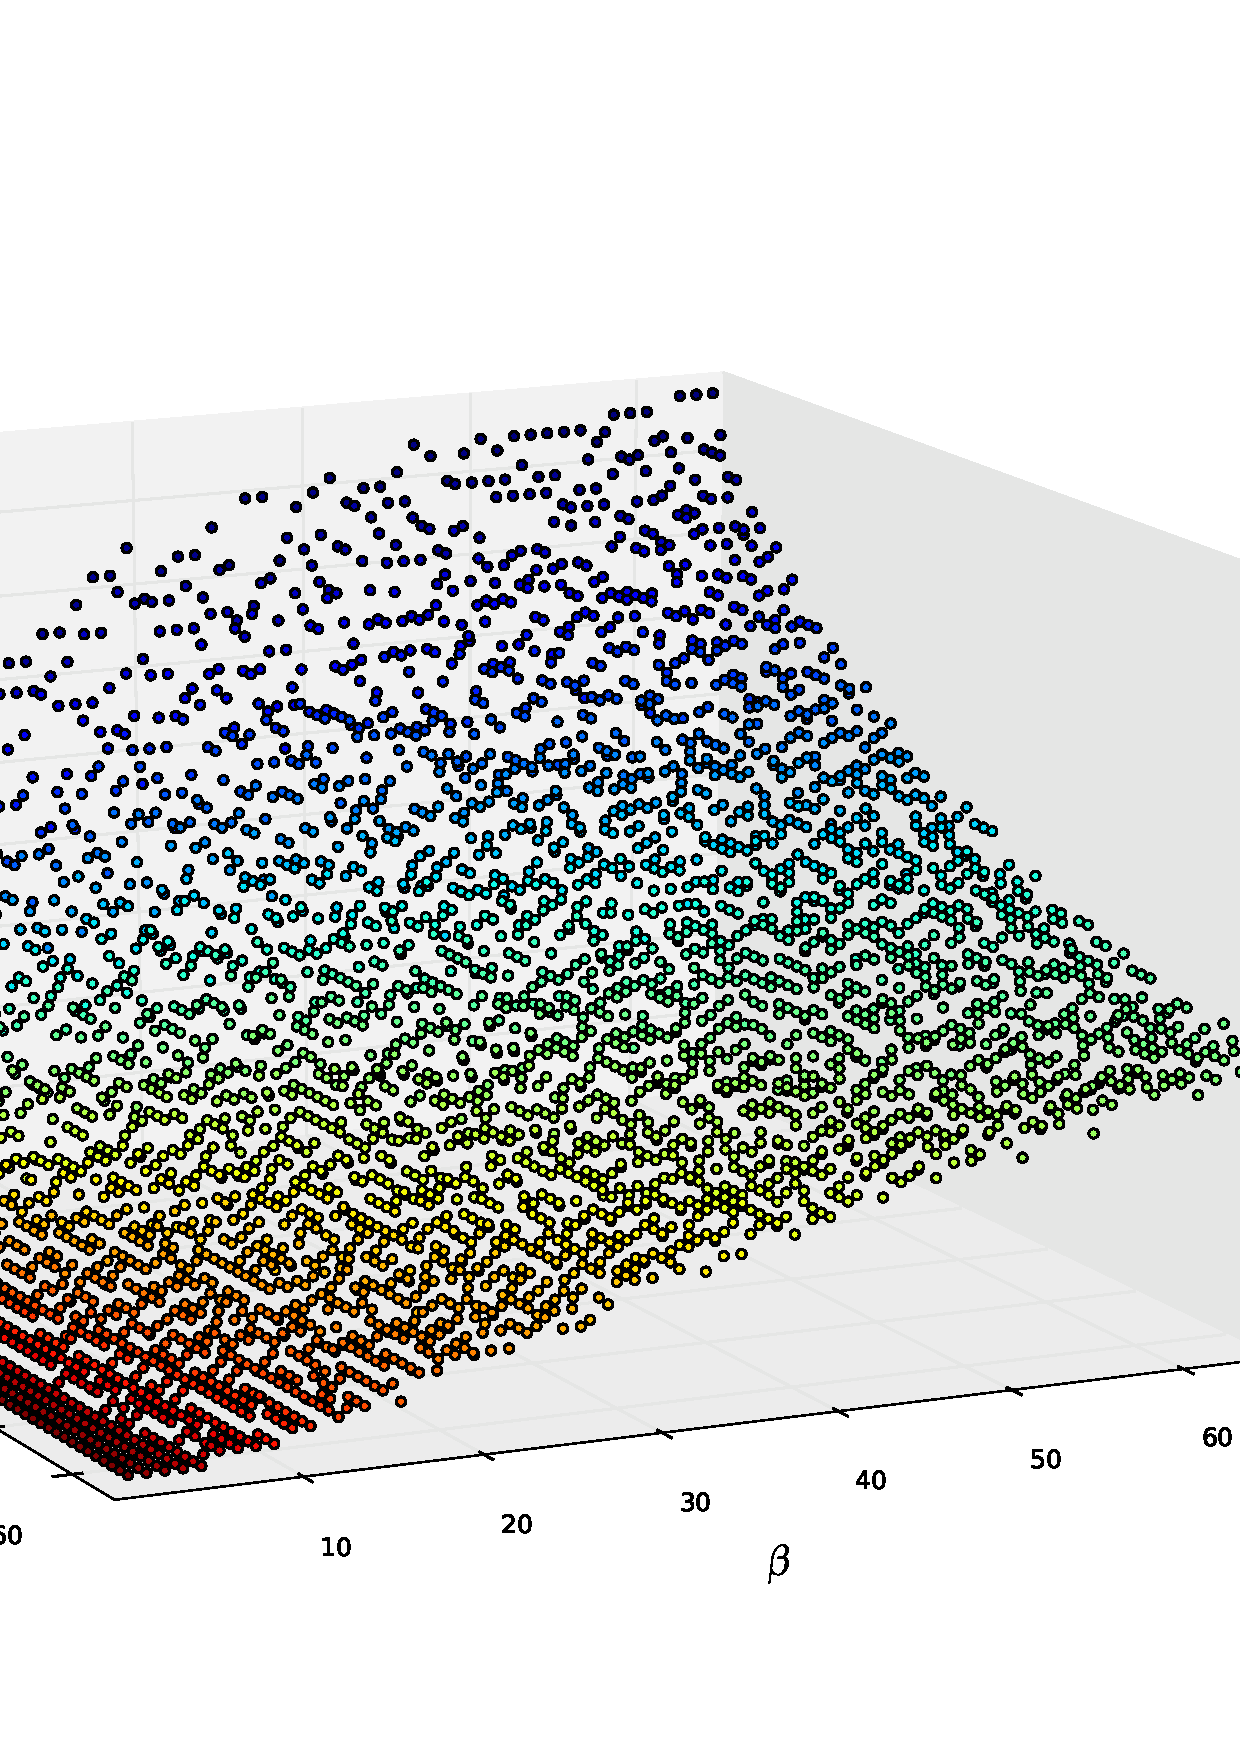
\includegraphics[scale=0.25,angle=-90]{fig05}
  }
  \caption{Histograms constructed from samples with 10,000 elements, generated 
from a Beta distribution. Below each histogram is possible to verify the 
parameters used.With these two parameters it is possible to perform different 
combinations of numbers to fill the arrays to be compressed.}
  \label{fig:02030405}
\end{figure}\todo{Adicionei a última frase}

\begin{figure}[h]
  \centering
   \subfigure[SM-VLB  Difference ($D = \eta_1 - \eta_2$)]{ 
    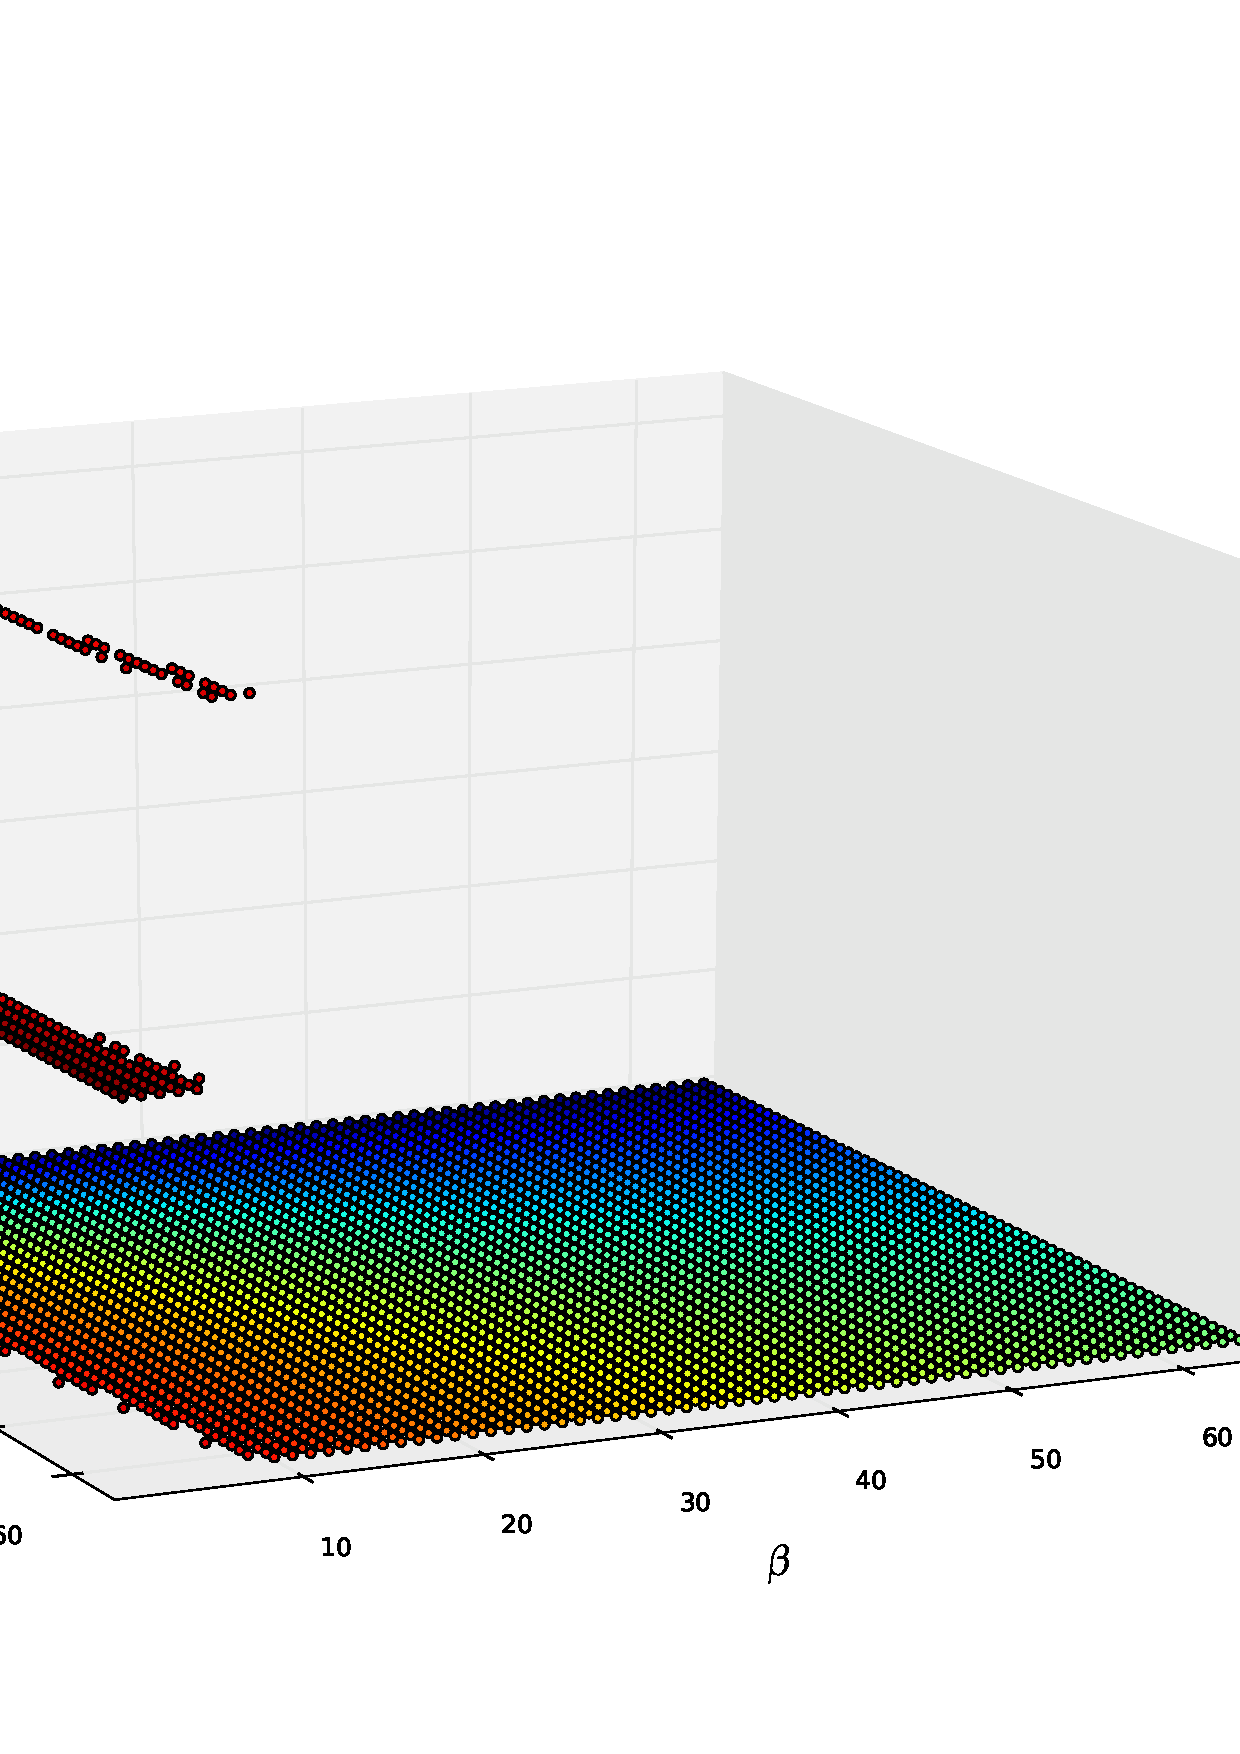
\includegraphics[scale=0.19,clip]{fig08}
   }
   \subfigure[SM Efficiency  ($\eta_1$)]{
    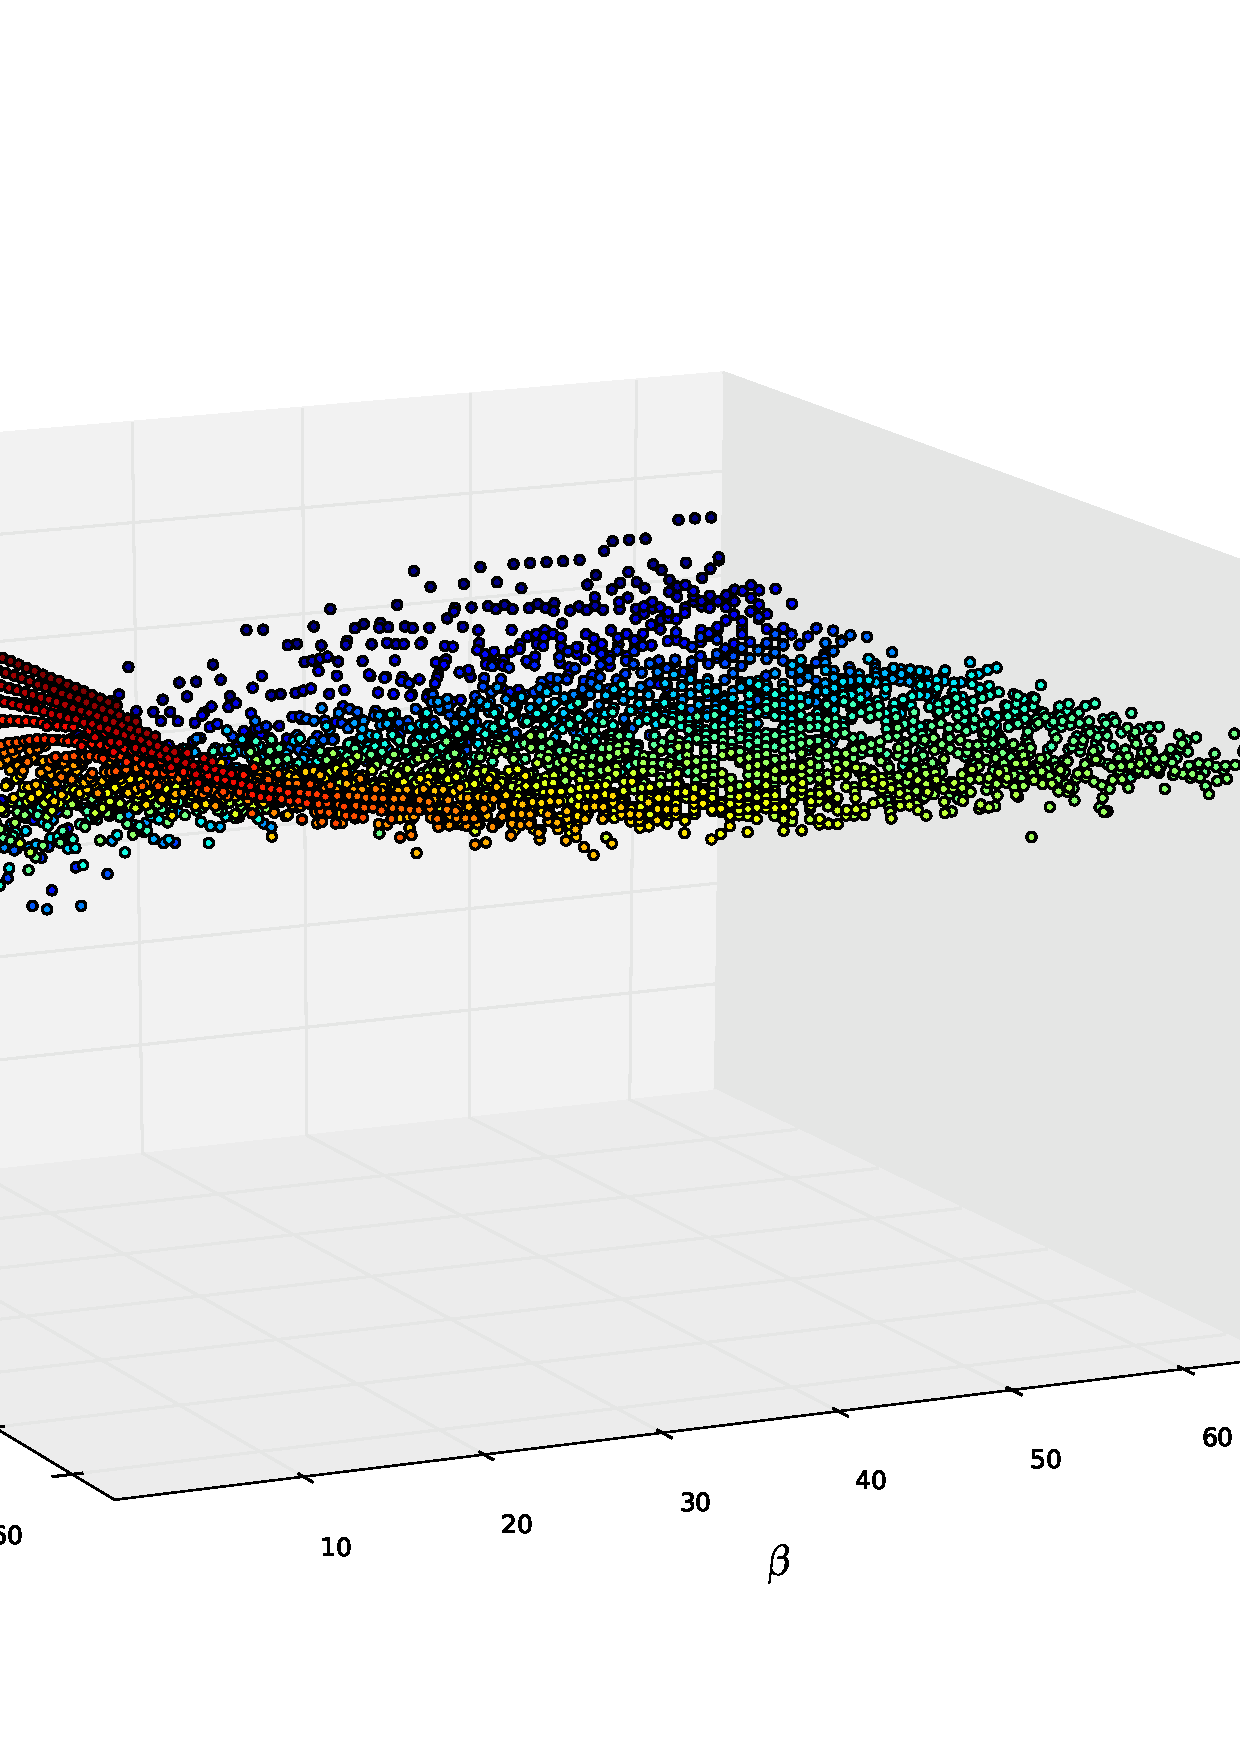
\includegraphics[scale=0.19,clip]{fig07}
   }
   \subfigure[VBL Efficiency ($\eta_2$)]{
    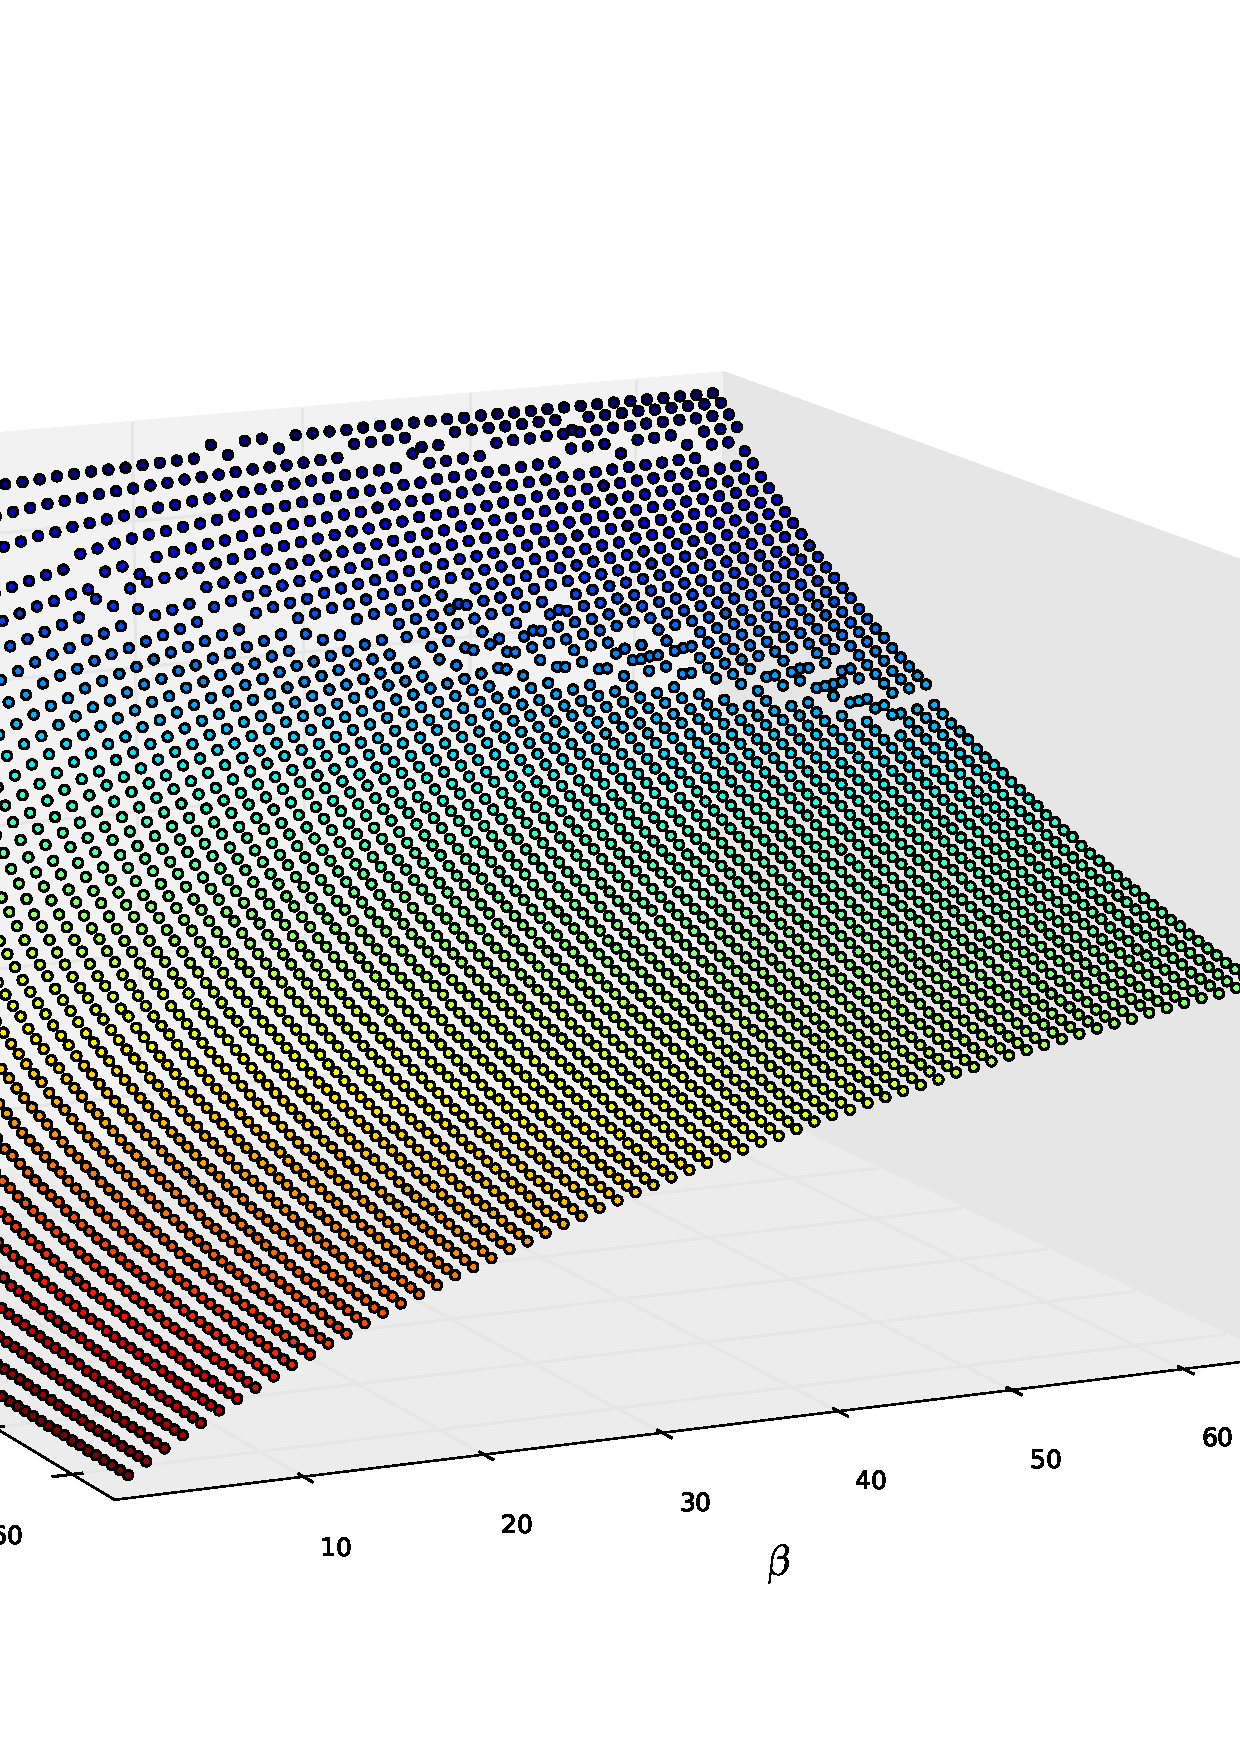
\includegraphics[scale=0.19,clip]{fig06}
   }
   \subfigure[SM$\geq$VLB Efficiency ($\eta_1 \geq \eta_2$)]{
    \includegraphics[scale=0.19,clip]{fig09}
   }
  \caption{Comparing compression efficiency of methods 1 and 2. Color scale in 
represent average bit-length. In (a) we can see the difference $D = \eta_1 - 
\eta_2$. It can be seen that for most combination of $\alpha$ and $\beta$, 
$D<0$, meaning the second method is more efficient to compress a sample of 
numbers with bit-lengths coming from a $Beta(\alpha,\beta)$ distribution. 
However, there is a small region in parameter space, which is shown in white on 
(d), where the SM method is more efficient. This region corresponds to the dots 
in red in (a), where the average bit-length is higher. In panels (b) and (c), we 
can see the efficiencies of SM and VLB methods, respectively.}
  \label{fig:06070809}
\end{figure}
\todo{A escala de cor é a mesma em todas as figuras, no texto estava dizendo 
que era apenas na a, b e c. Eu alterei.}

\begin{figure}[h]
  \centering
  \subfigure[$\alpha_1=1,\beta_1=1,\alpha_2=1,\beta_2=1$]{
   \includegraphics[scale=0.28,angle=-90,clip]{fig10}
  }
  \subfigure[$\alpha_1=1,\beta_1=32,\alpha_2=32,\beta_2=1$]{
   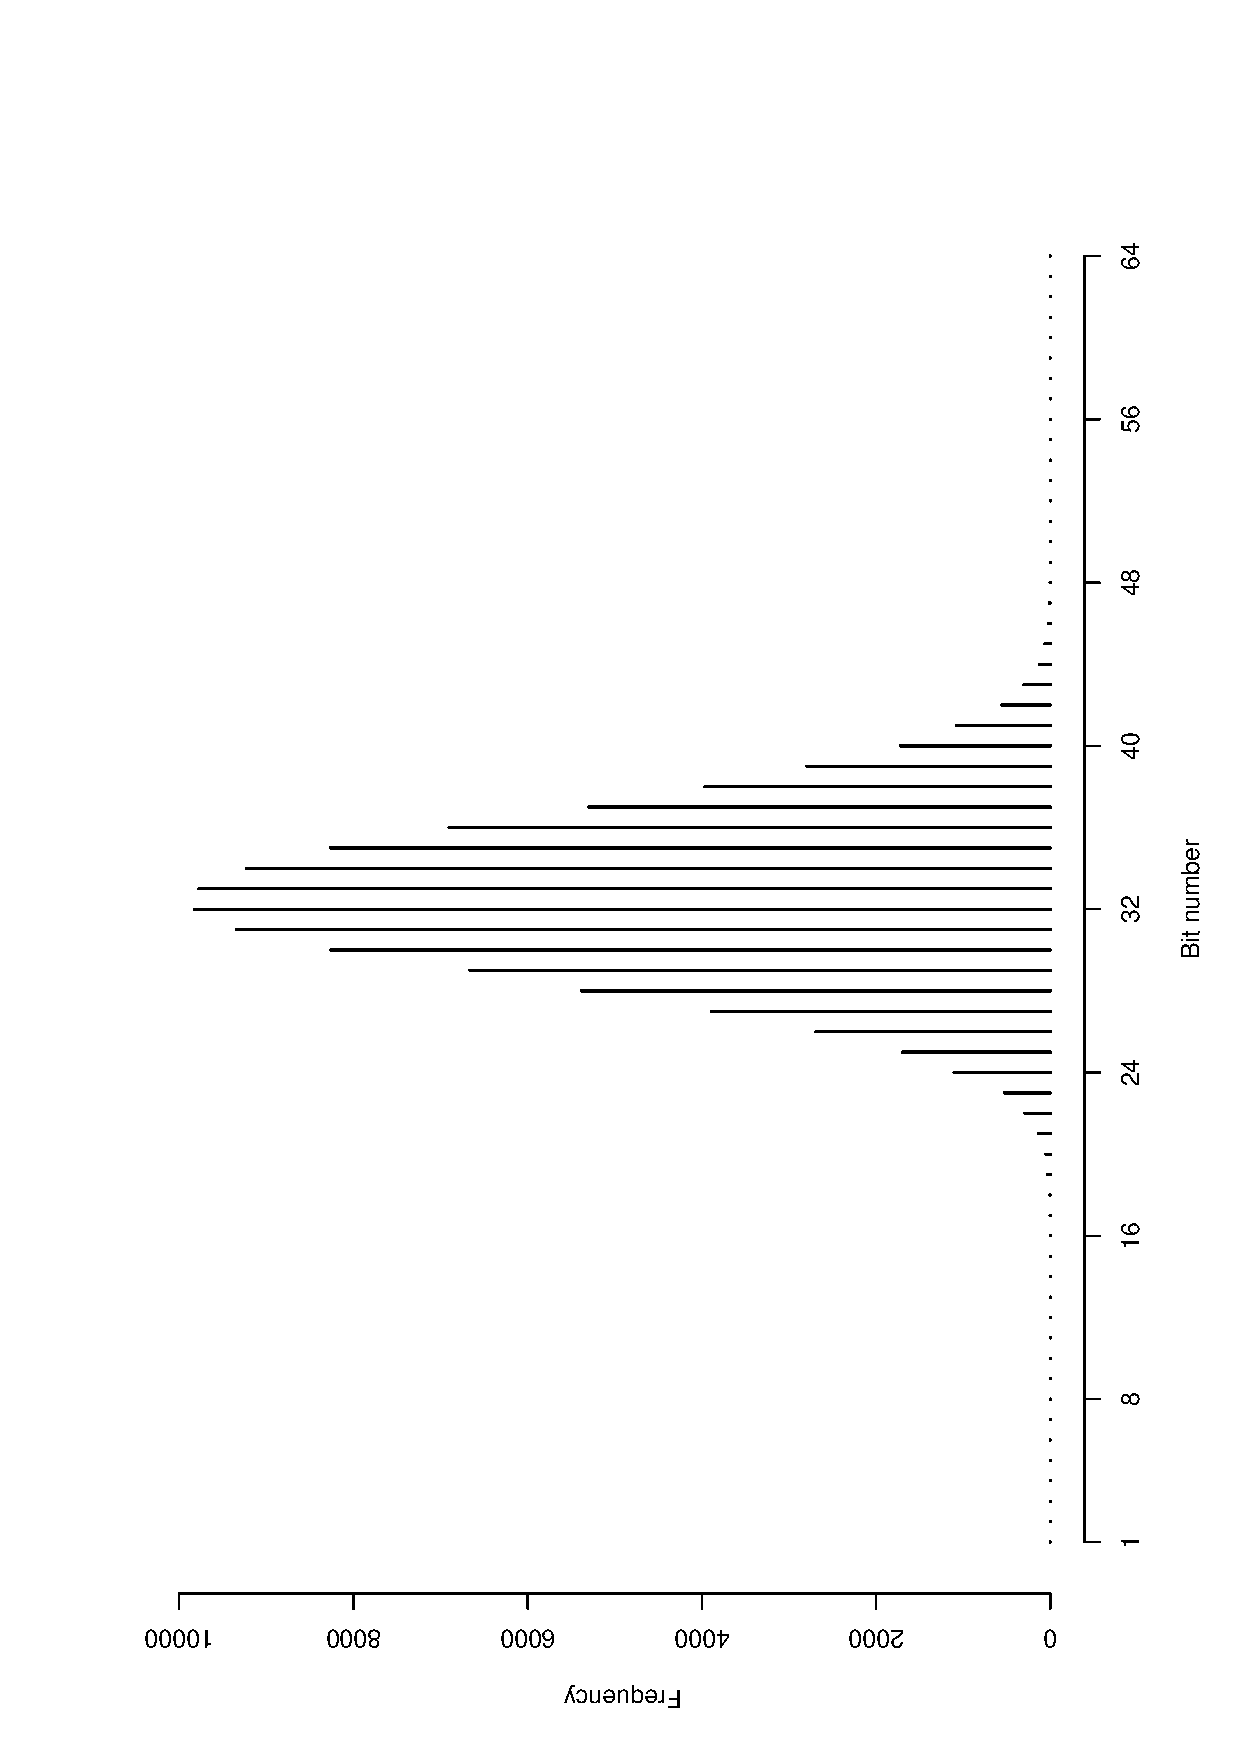
\includegraphics[scale=0.28,angle=-90,clip]{fig11}
  }
  \subfigure[$\alpha_1=32,\beta_1=32,\alpha_2=32,\beta_2=32$]{
   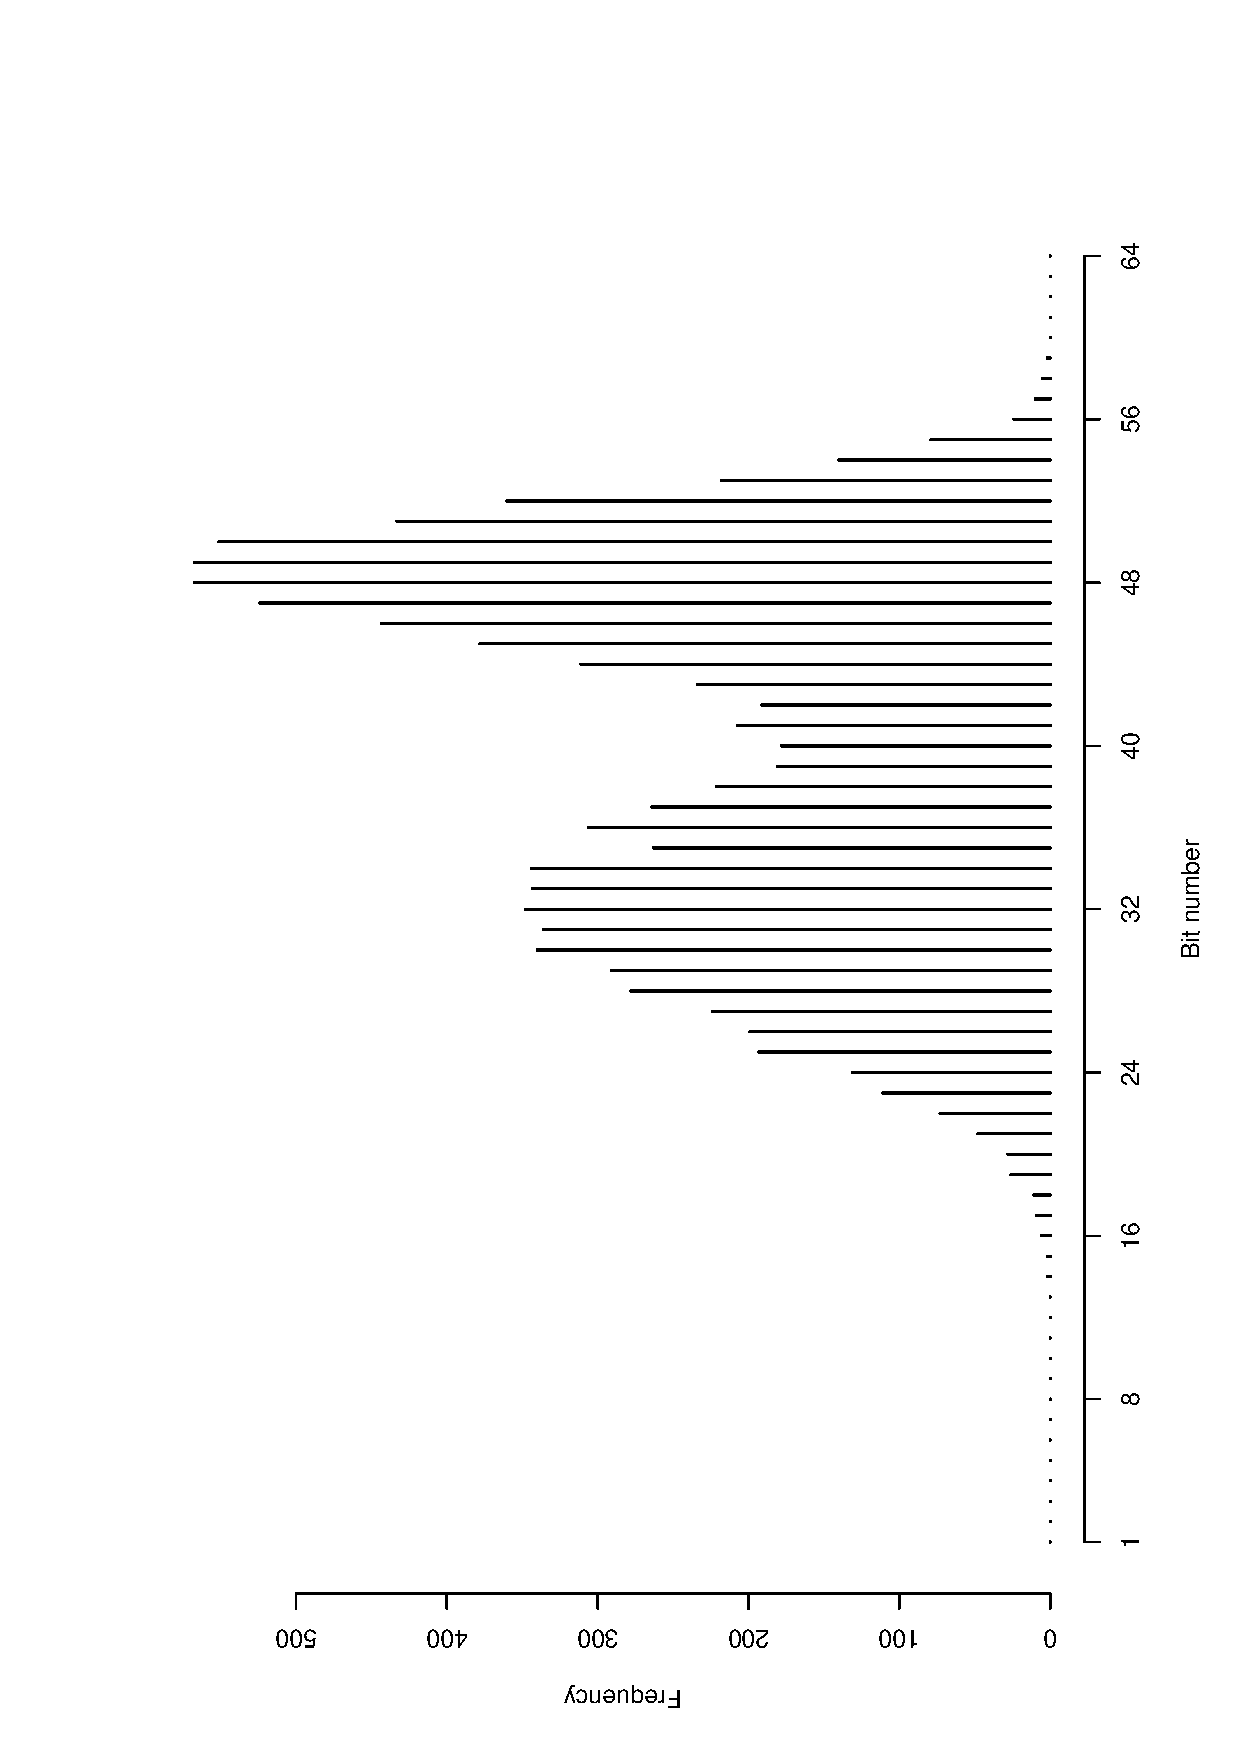
\includegraphics[scale=0.28,angle=-90,clip]{fig12}
  }
  \subfigure[$\alpha_1=64,\beta_1=32,\alpha_2=32,\beta_2=64$]{
   \includegraphics[scale=0.28,angle=-90]{fig13}
  }
  \caption{Histograms constructed from samples with 10,000 elements, generated 
from the mixture of two Beta distributions with $w=0.5$. Below each histogram 
are the parameters of the mixture.}
  \label{fig:10111213}
\end{figure}

\begin{figure}[h]
  \centering
  \subfigure[$\alpha_1=64,\beta_1=48,\alpha_2=1,\beta_2=48$]{
   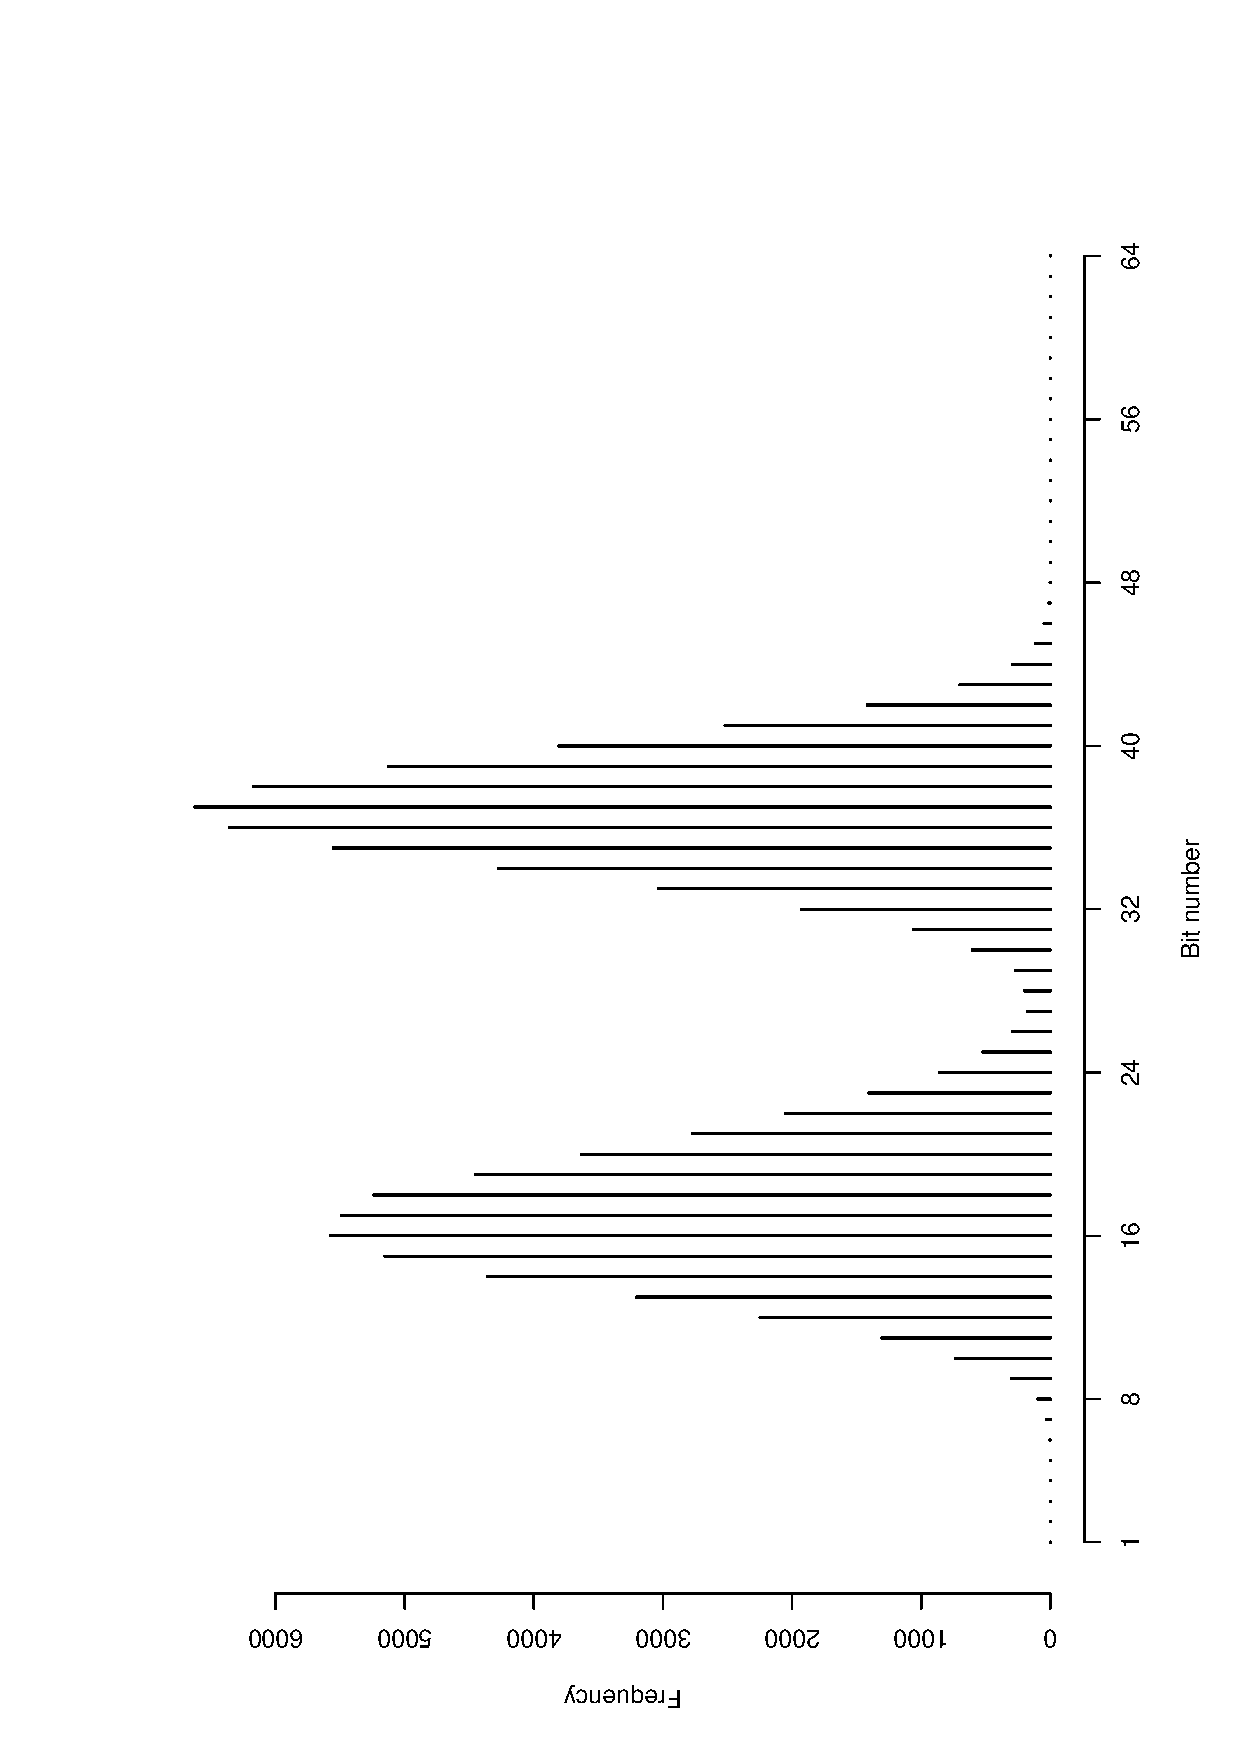
\includegraphics[scale=0.28,angle=-90]{fig14}
  }
  \subfigure[$\alpha_1=16,\beta_1=46,\alpha_2=49,\beta_2=64$]{
   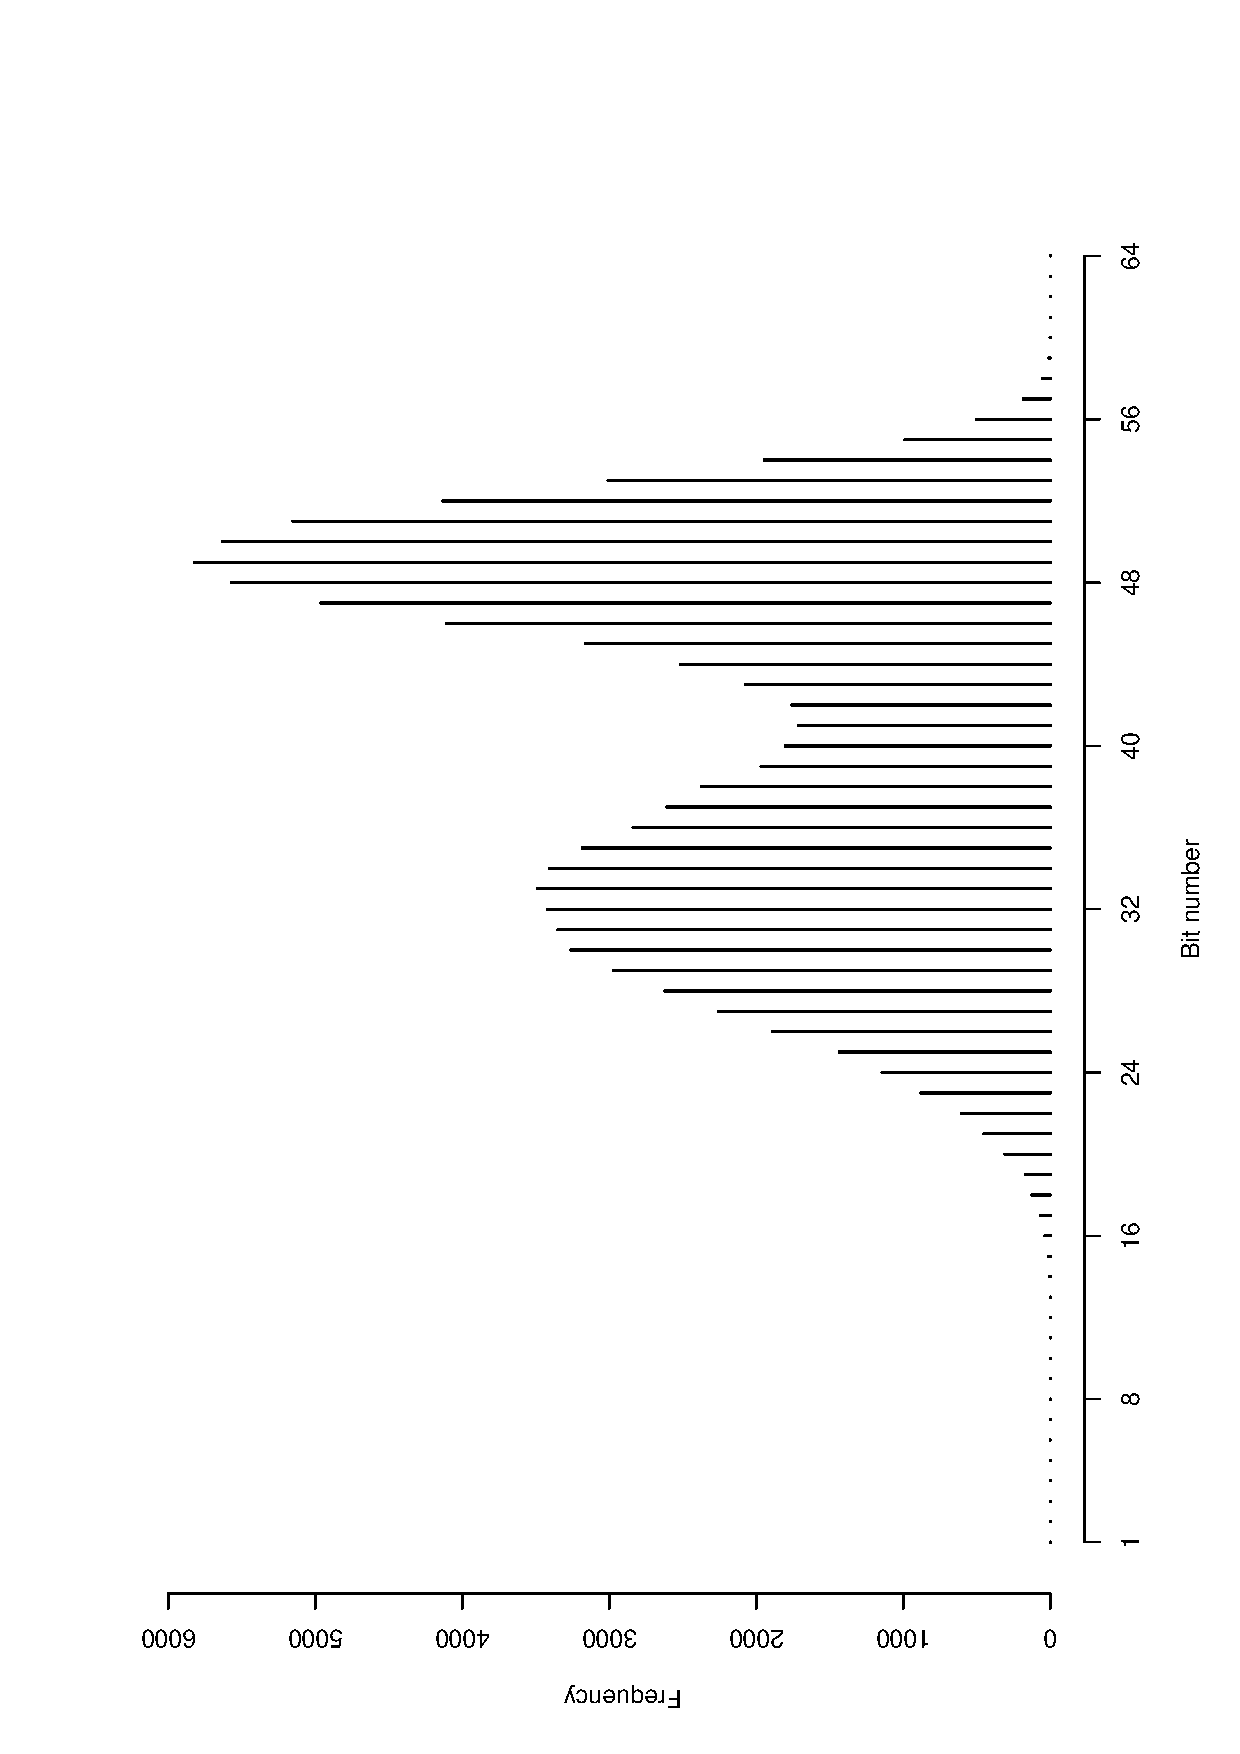
\includegraphics[scale=0.28,angle=-90]{fig15}
  }
  \subfigure[$\alpha_1=16,\beta_1=16,\alpha_2=16,\beta_2=49$]{
   \includegraphics[scale=0.28,angle=-90]{fig16}
  }
  \subfigure[$\alpha_1=1,\beta_1=16,\alpha_2=1,\beta_2=49$]{
   \includegraphics[scale=0.28,angle=-90]{fig17}
  }
  \caption{Histograms constructed from samples with 10,000 elements, generated 
from the mixture of two Beta distributions with $w=0.5$. Below each histogram 
are the parameters of the mixture.}
  \label{fig:14151617}
\end{figure}

\begin{figure}[h]
  \centering
  \subfigure[Efficiency histogram of the SM method ]{
   \includegraphics[scale=0.25,angle=-90]{fig18}
  \label{fig:18}
  }
  \subfigure[Efficiency histogram of the VLB method ]{
   \includegraphics[scale=0.25,angle=-90]{fig19}
  \label{fig:19}
  }
  \caption{Efficiency histograms of the SM and VLB methods. Note that the VLB 
method has a greater average efficiency than SM method.}
  \label{fig:1819}
\end{figure}

\begin{figure}[h]
  \centering
   \subfigure[Efficiencies of the SM and VLB methods, for constant bit-length 
matrices.]{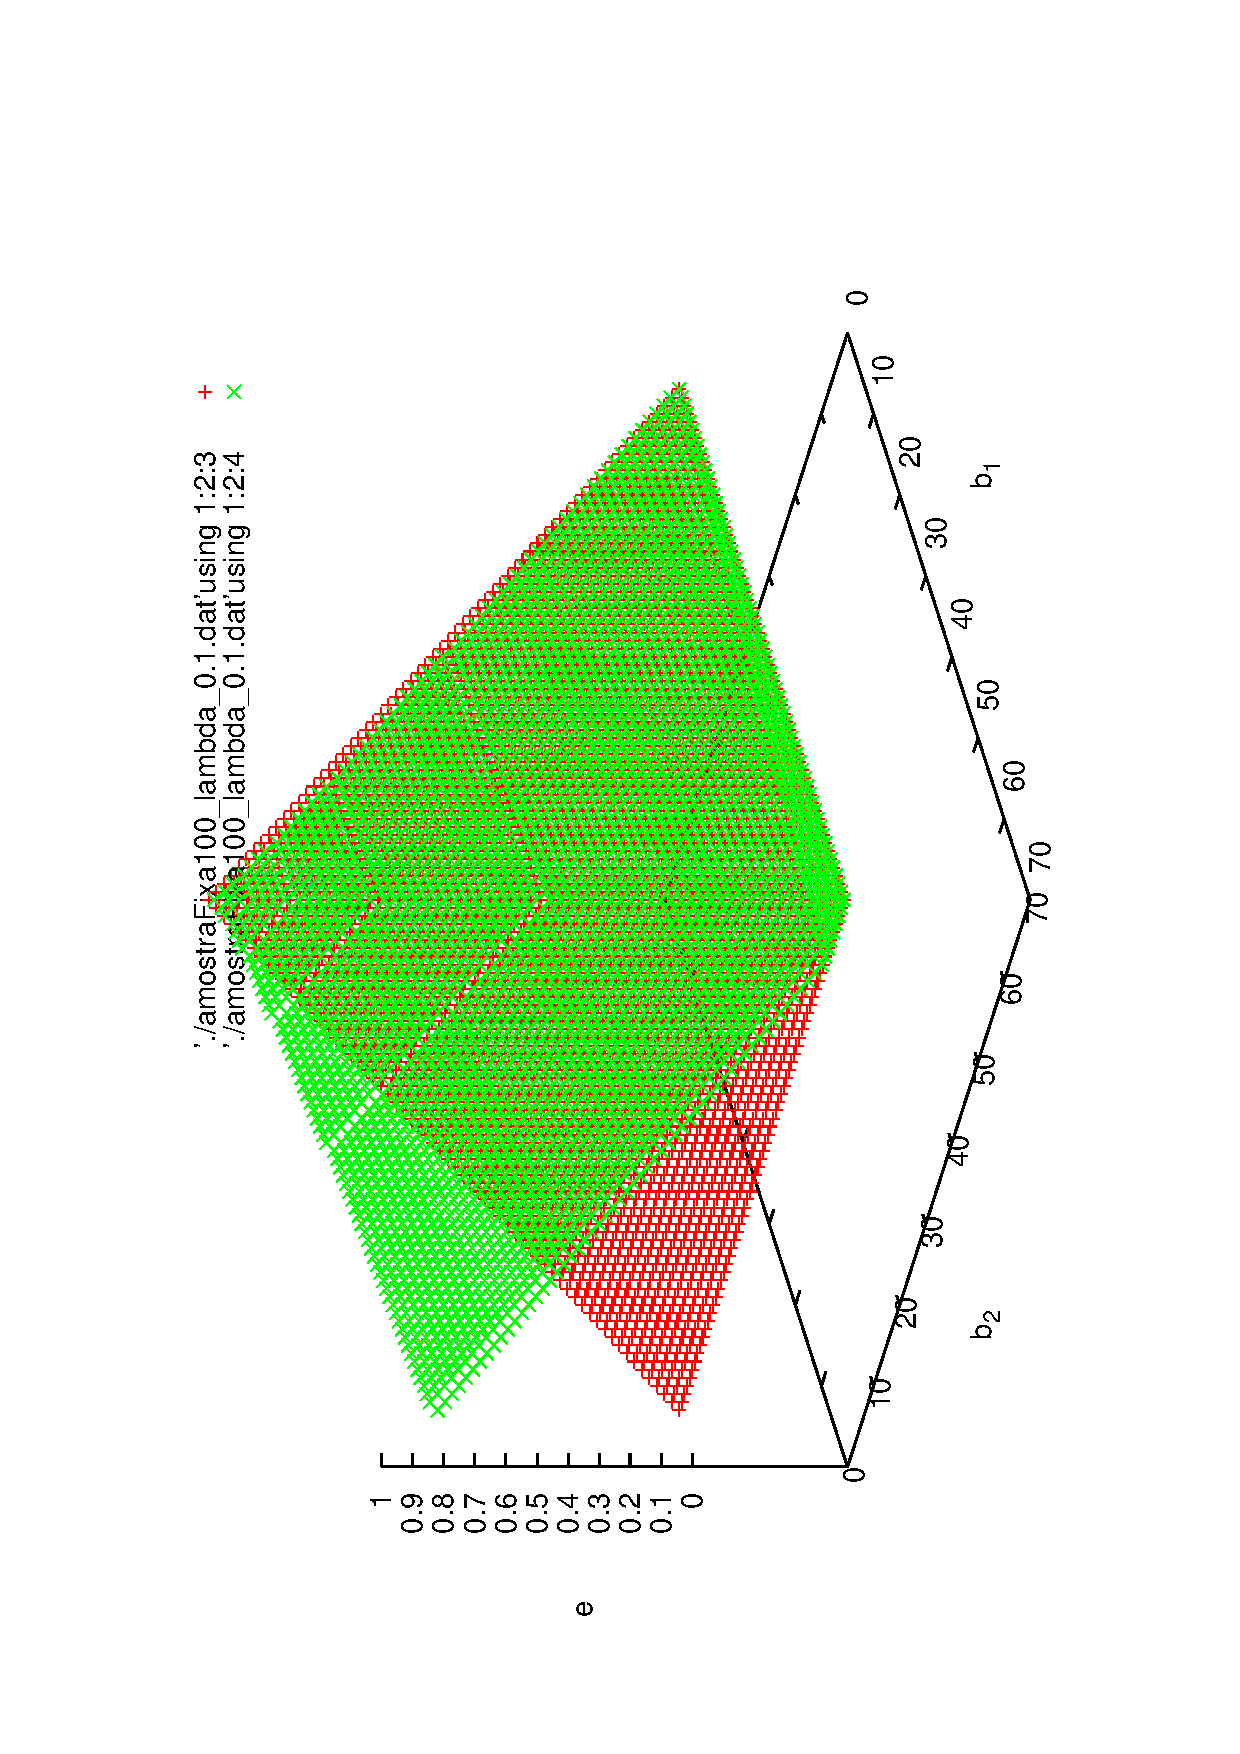
\includegraphics[scale=0.3,clip]{fig20}\label{fig20}}
   \subfigure[$\eta_1-\eta_2$ for matrices of constant 
bit-length.]{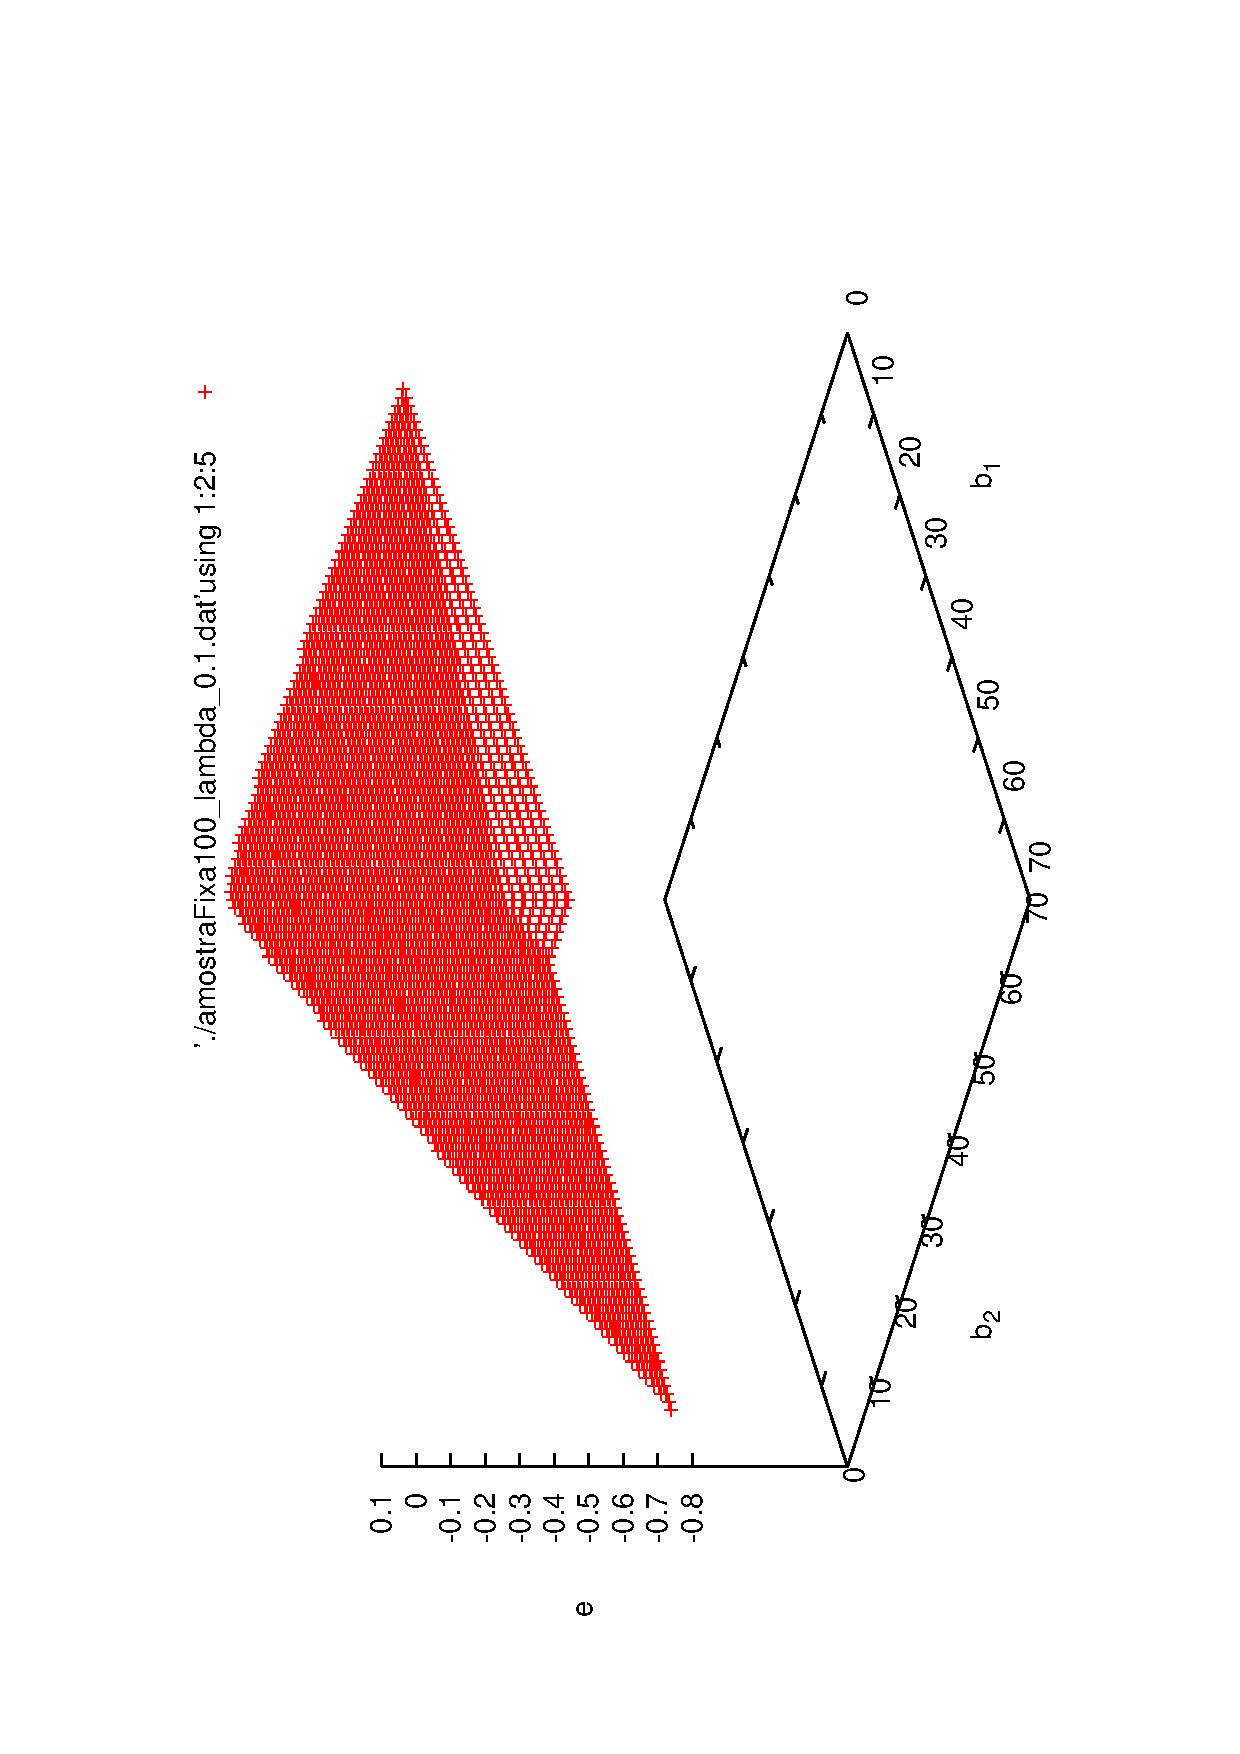
\includegraphics[scale=0.3,clip]{fig21}\label{fig21}}
  \caption{Compression efficiency of the SM and VLB methods for matrices of 
constant bit-length.}
  \label{fig:2021}
\end{figure}

\begin{figure}[h]
  \centering
  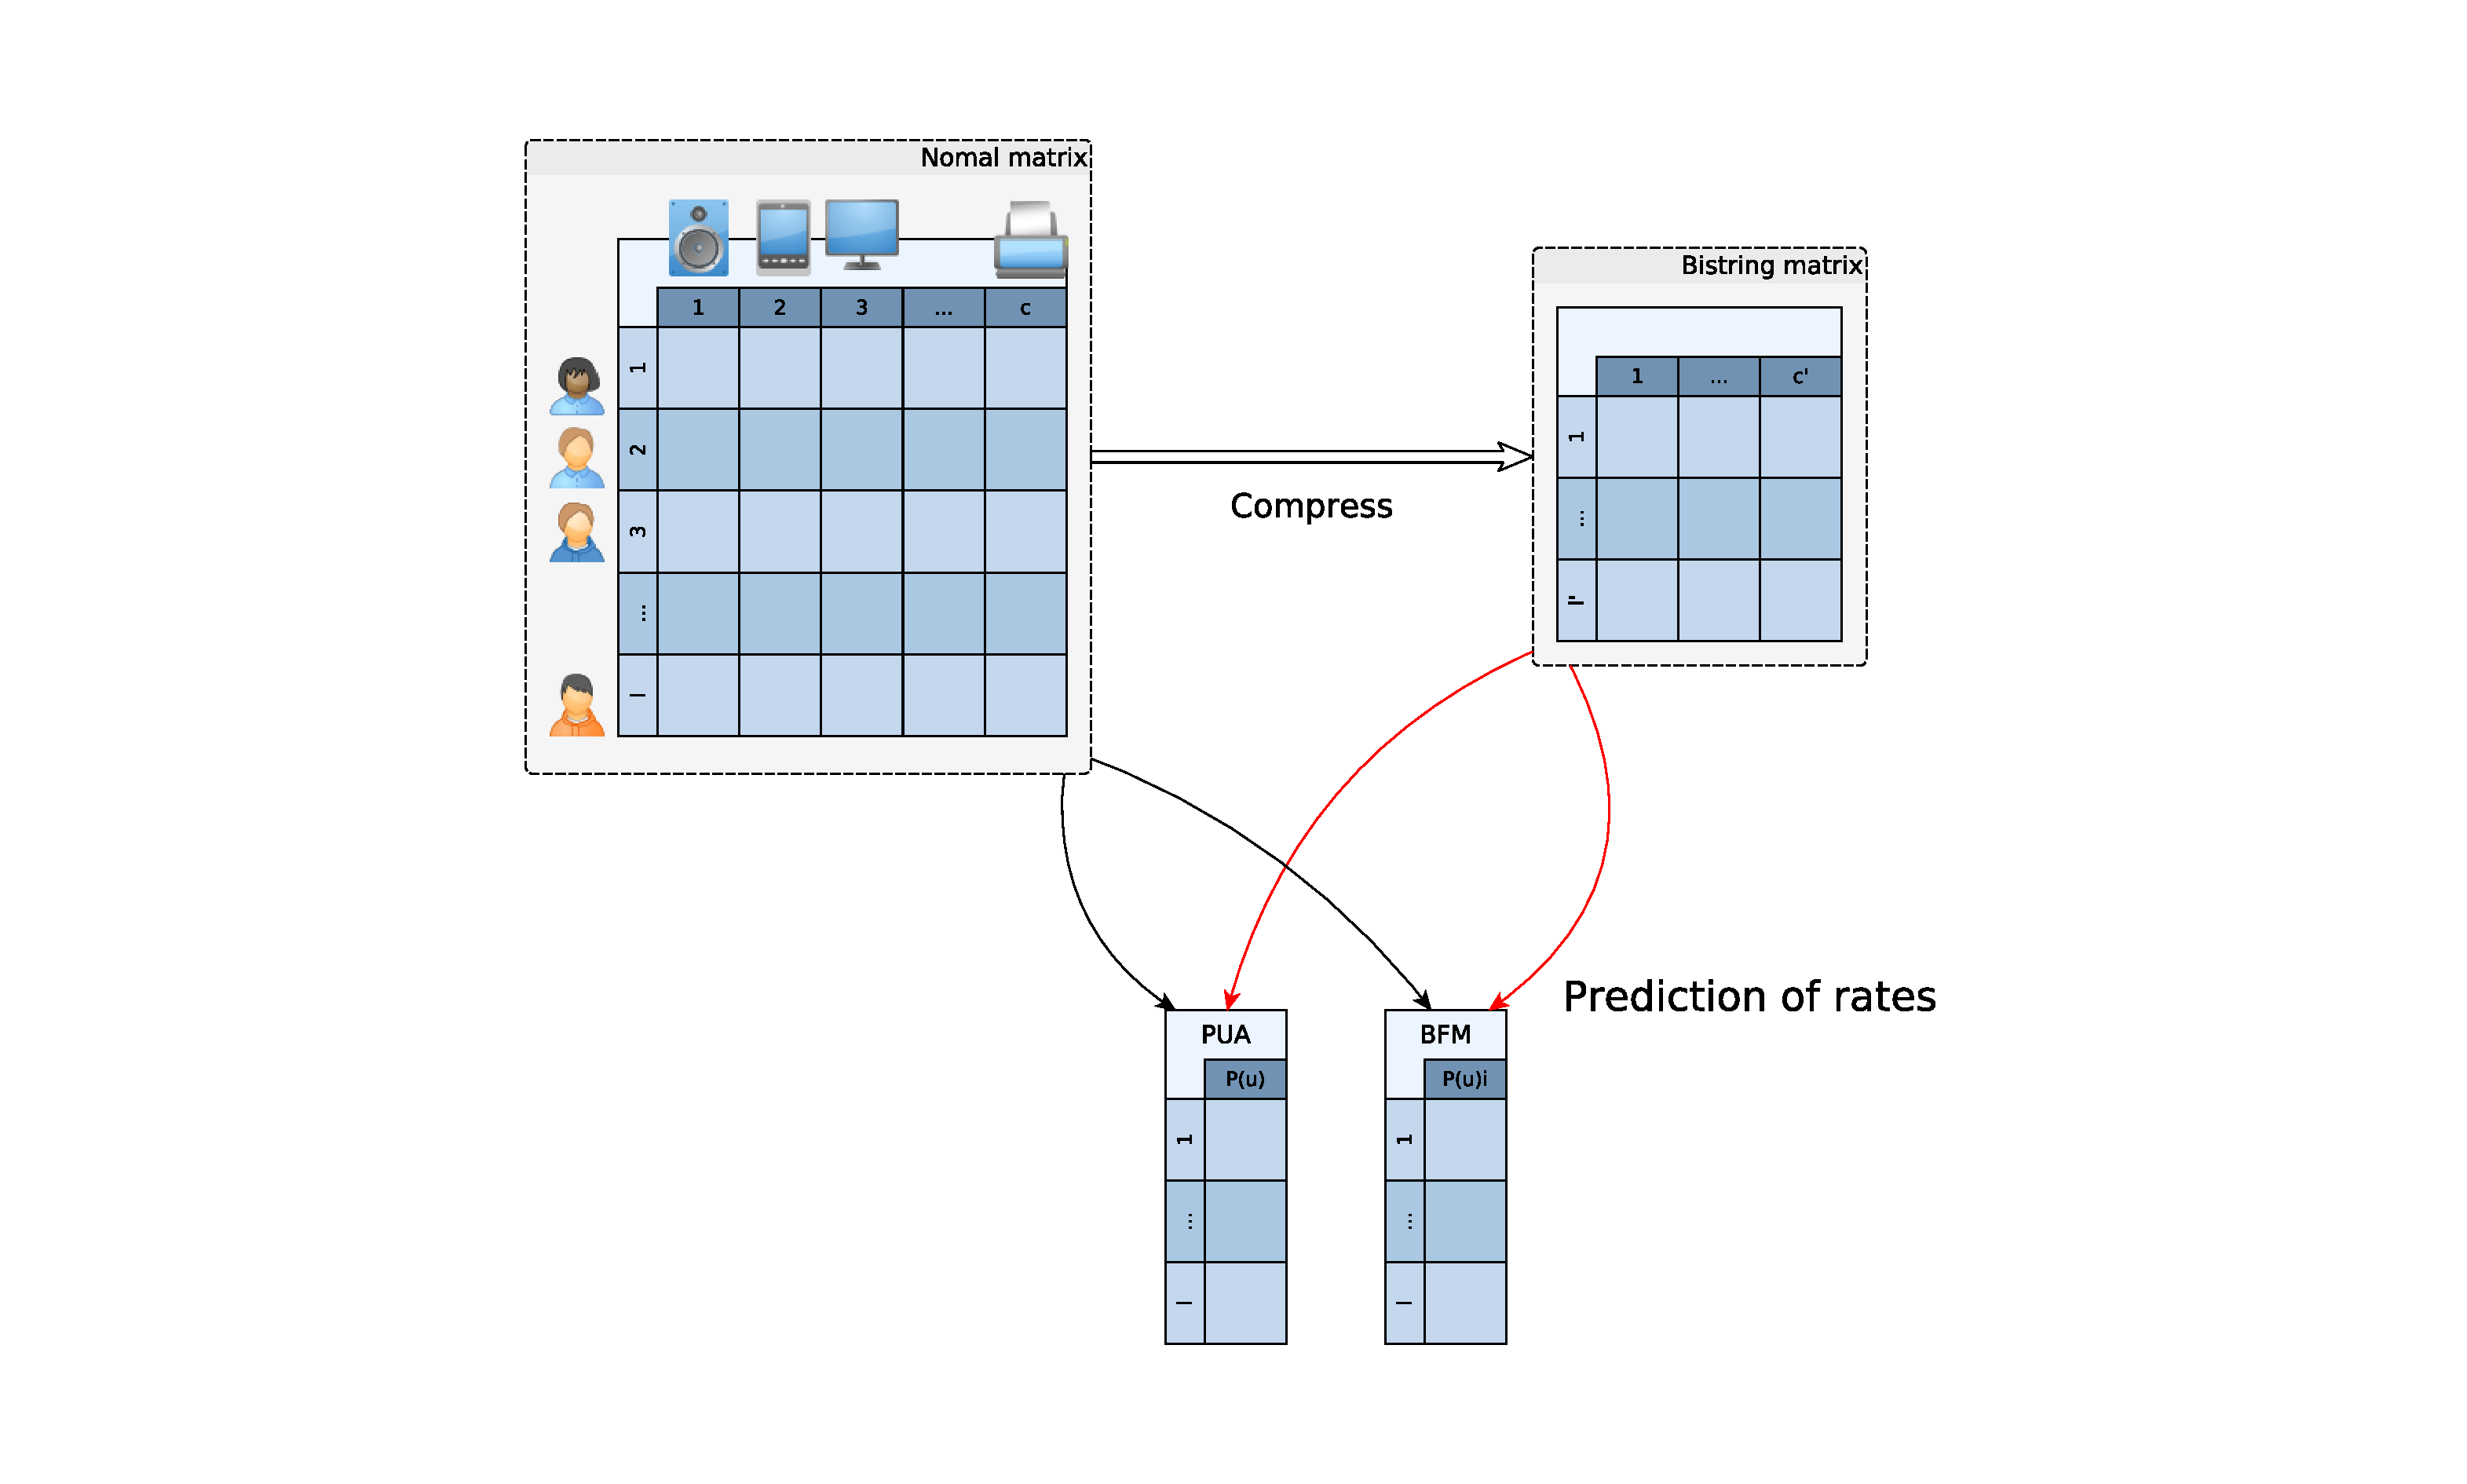
\includegraphics[scale=0.4,trim=5cm 0cm 5cm 0cm,clip]{fig22}
  \caption{Illustration of the process of the bistring model application to matrices of collaborative filttering of the 
algorithms per use average (PUA) and of the bias from mean (BFM) in a matrix represented in the traditional and 
bitstring formats.}
  \label{fig22}
\end{figure}


\begin{figure}[h]
  \centering
  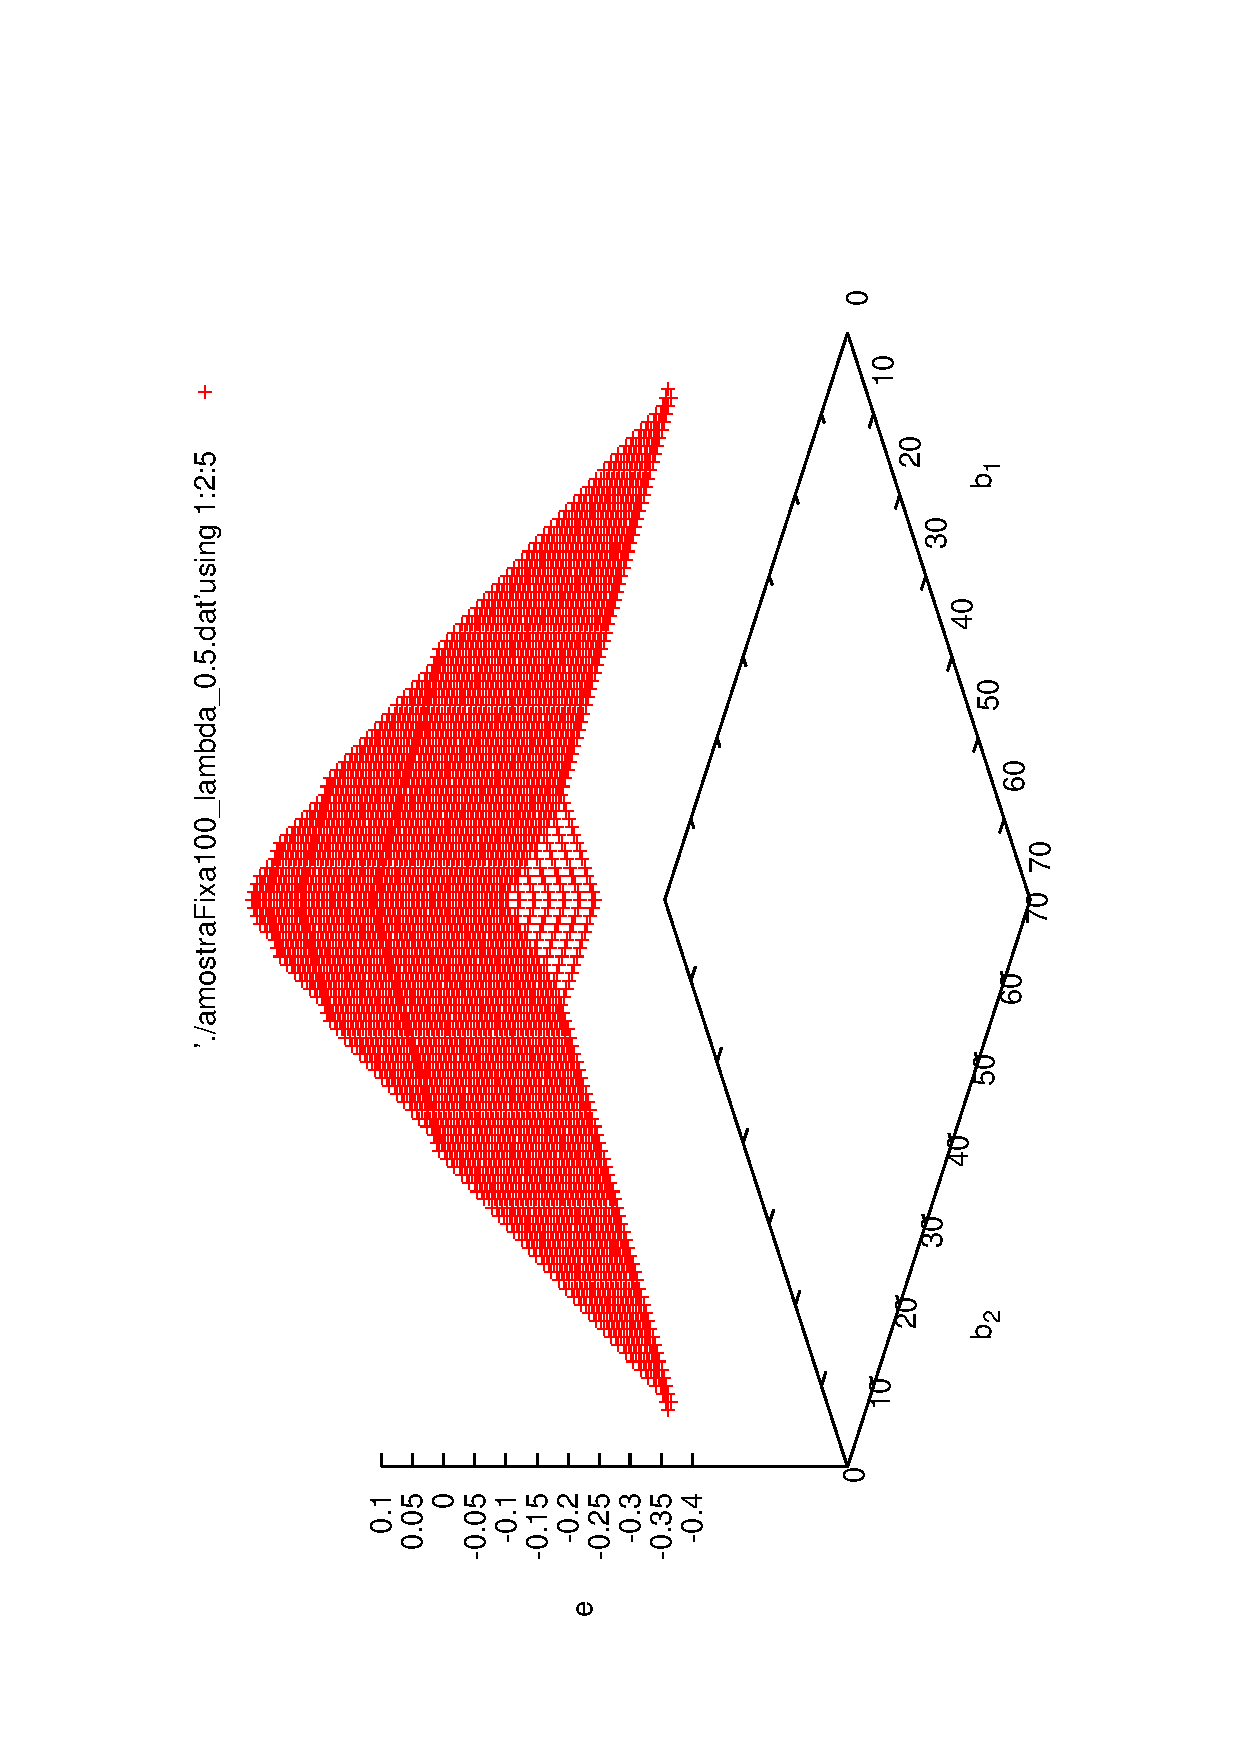
\includegraphics[scale=0.6,clip]{fig23}
  \caption{Tempo de processamento do método Per User Average em função do número de linhas de uma matriz com 3,000 
colunas. A linha verde na vetical indica que o momento aproximado que o método tradicional demanda acesso a disco para 
armazenar a matriz a ser analisada, onerando o processo. O método de bitstring consegue representar a matriz 
integralmente na memória, sem a necessiada de acesso a disco.}
  \label{fig23}
\end{figure}

\begin{figure}[h]
  \centering
  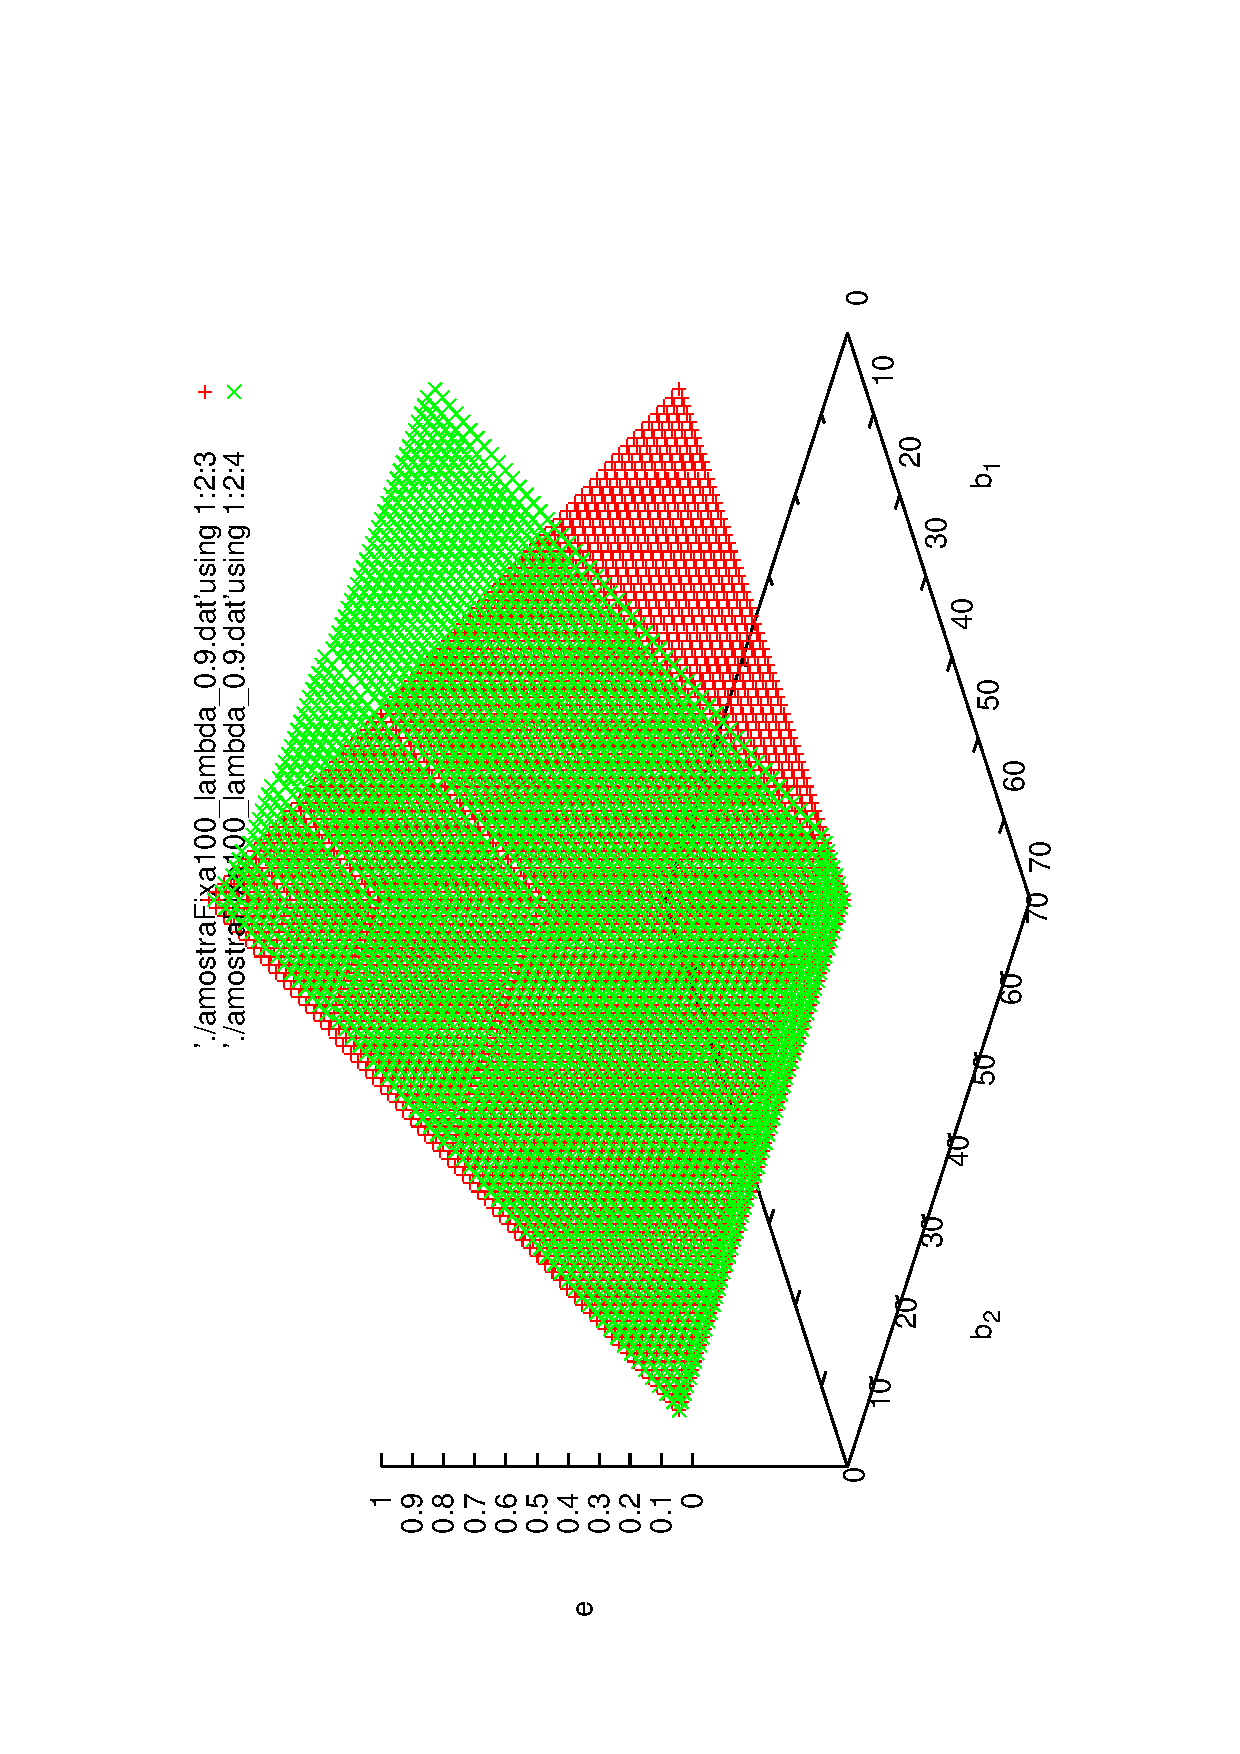
\includegraphics[scale=0.6,clip]{fig24}
  \caption{Tempo de processamento do método Per User Average em função do número de linhas de uma matriz com 3,000 
colunas. A linha verde na vetical indica que o momento aproximado que o método tradicional demanda acesso a disco para 
armazenar a matriz a ser analisada, onerando o processo. Para dimensões inferiores a aproximadamente 400 liinhas, o 
método tracional é mais rápido que o de bitstring, ressaltando que o custo computacional dos dois métodos é linear.}
  \label{fig24}
\end{figure}

\begin{figure}[h]
  \centering
  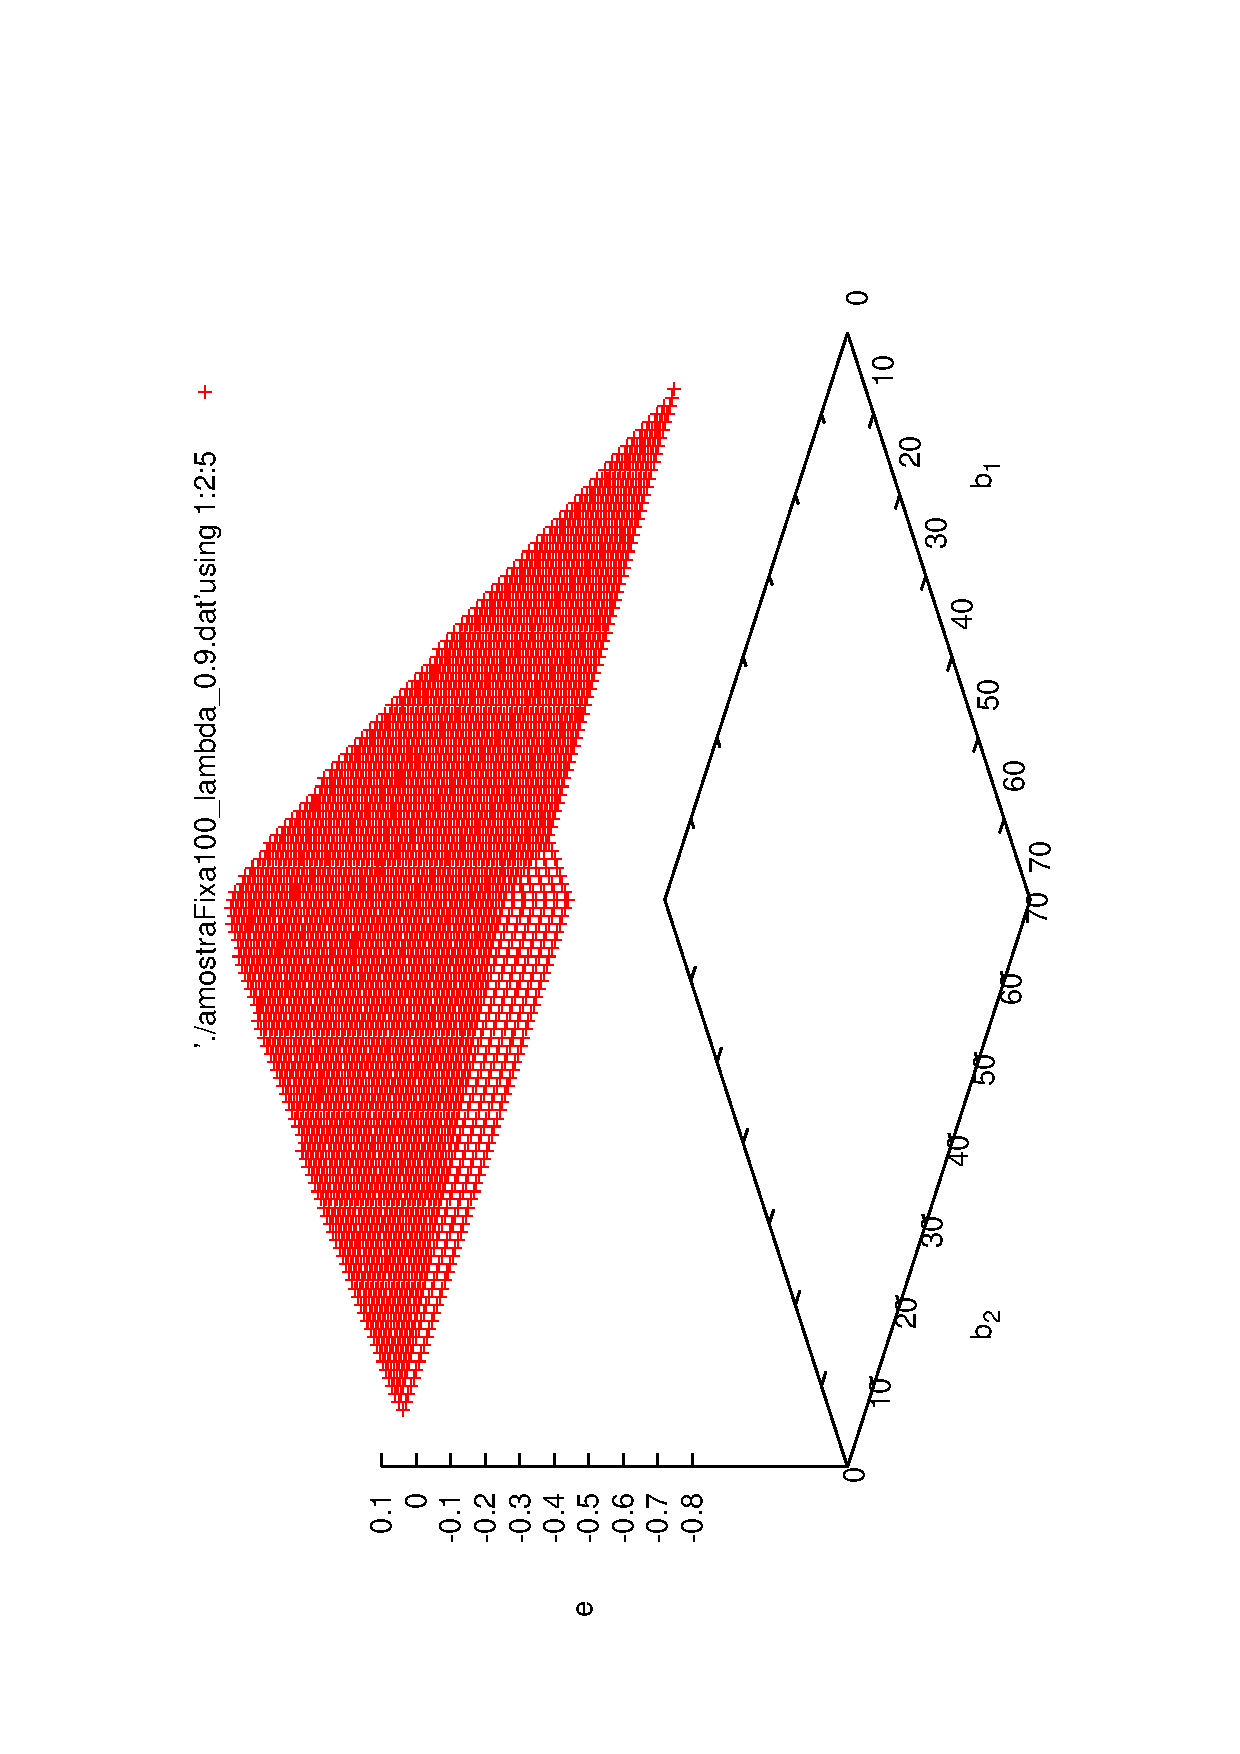
\includegraphics[scale=0.6,clip]{fig25}
  \caption{Relação entre o tempo de processamento pelo método de bisttring e o método tracional em função do número de 
linhas de uma matriz com 3,000 colunas. Verifica-se que para a matriz com um número inferior a aproximadamente 400 
linhas, o método tradicional é mais rápido, porém quando o número de linhas é superior, o método de bitstring é mais 
rápido, por causa da representação compactada em  memória da matriz.}
  \label{fig25}
\end{figure}

\begin{figure}[h]
  \centering
  \includegraphics[scale=0.6,clip]{fig26}
  \caption{xxx.}
  \label{fig23}
\end{figure}

\begin{figure}[h]
  \centering
  \includegraphics[scale=0.6,clip]{fig27}
  \caption{xxx.}
  \label{fig24}
\end{figure}

\begin{figure}[h]
  \centering
  \includegraphics[scale=0.6,clip]{fig28}
  \caption{xxx.}
  \label{fig25}
\end{figure}



\begin{figure}[h]
  \centering
  \subfigure[$A=5$]{
  \includegraphics[scale=0.4,clip]{fig29}
  }
  \subfigure[$A=A+5$]{
  \includegraphics[scale=0.4,clip]{fig30}
  }
  \subfigure[$A=A+A$]{
  \includegraphics[scale=0.4,clip]{fig31}
  }
  \subfigure[$A=A-8$]{
  \includegraphics[scale=0.4,clip]{fig32}
  }
  \caption{Z}
  \label{fig:29303132}
\end{figure}

\begin{figure}[h]
  \centering
  \subfigure[$A=5$]{
  \includegraphics[scale=0.4,clip]{fig33}
  }
  \subfigure[$A=A+5$]{
  \includegraphics[scale=0.4,clip]{fig34}
  }
  \subfigure[$A=A+A$]{
  \includegraphics[scale=0.4,clip]{fig35}
  }
  \subfigure[$A=A-8$]{
  \includegraphics[scale=0.4,clip]{fig36}
  }
  \caption{Z}
  \label{fig:33343536}
\end{figure}

\begin{figure}[h]
  \centering
  \subfigure[$A=5$]{
   \includegraphics[scale=0.4,clip]{fig37}
  }
  \subfigure[$A=A+5$]{
   \includegraphics[scale=0.4,clip]{fig38}
  }
  \subfigure[$A=A+A$]{
   \includegraphics[scale=0.4,clip]{fig39}
  }
  \subfigure[$A=A-8$]{
   \includegraphics[scale=0.4,clip]{fig40}
  }
  \caption{R}
  \label{fig:37383940}
\end{figure}

\begin{figure}[h]
  \centering
  \subfigure[$A=5$]{
   \includegraphics[scale=0.4,clip]{fig41}
  }
  \subfigure[$A=A+5$]{
   \includegraphics[scale=0.4,clip]{fig42}
  }
  \subfigure[$A=A+A$]{
   \includegraphics[scale=0.4,clip]{fig43}
  }
  \subfigure[$A=A-8$]{
   \includegraphics[scale=0.4,clip]{fig44}
  }
  \caption{R}
  \label{fig:41424344}
\end{figure}



%\begin{figure}[!ht]
%\begin{center}
%%\includegraphics[width=4in]{figure_name.2.eps}
%\end{center}
%\caption{
%{\bf Bold the first sentence.}  Rest of figure 2  caption.  Caption 
%should be left justified, as specified by the options to the caption 
%package.
%}
%\label{Figure_label}
%\end{figure}

\newpage

\section*{Tables}
%\begin{table}[!ht]
%\caption{
%\bf{Table title}}
%\begin{tabular}{|c|c|c|}
%table information
%\end{tabular}
%\begin{flushleft}Table caption
%\end{flushleft}
%\label{tab:label}
% \end{table}

\begin{table}[h]
 \centering
 \caption{The first 8 elements of $M$ represented in binary base.}
 \begin{tabular}{cccc} 
  \hline 
  Element & Value  & Binary & Bit length\\
  \hline
  $M_{1,1}$ & 900  & 1110000100 & 10\\
  $M_{1,2}$ & 1023 & 1111111111 & 10\\
  $M_{1,3}$ & 721  & 1011010001 & 10\\
  $M_{1,4}$ & 256  & 100000000  & 9\\
  $M_{1,5}$ & 1    & 1          & 1\\
  $M_{1,6}$ & 10   & 1010       & 4\\
  $M_{1,7}$ & 700  & 1010111100 & 10\\
  $M_{1,8}$ & 20   & 10100      & 5\\
  \hline
 \end{tabular}
 \label{tab:01}
\end{table}

\begin{table}[h]
 \centering
 \caption{Efficiency comparison of SM and VLB methods for parameters covering 
uniformly the support of $B$. Column $n$ shows the number of parameter 
combinations with which each method has superior compression.}
 \begin{tabular}{crr}
  \hline 
  Methods  & n   & Percentage \\
  \hline
  SM	   & 592	& 0.9034\% \\
  VLB	   & 64944	& 99.0966\% \\
  \hline
  Total    & 65536	& 100\% \\
  \hline
 \end{tabular}
 \label{tab:02}
\end{table}

\begin{table}[h]
 \centering
 \caption{Combinations $p_1$ and $p_2$ to calculate the efficiency.}
 \begin{tabular}{ccc}
  \hline 
  $p_1$  & $p_2$ & $\eta_2$ \\
  \hline
  0.0	&1.0    &-0.109 \\
  0.1	&0.9	&-0.010 \\
  0.2	&0.8	&0.087 \\
  0.3	&0.7	&0.185 \\
  0.4	&0.6	&0.284 \\
  0.5	&0.5	&0.382 \\
  0.6	&0.4	&0.481 \\
  0.7	&0.3	&0.579 \\ 
  0.8	&0.2	&0.678 \\
  0.9	&0.1	&0.776 \\ 
  1.0	&0.0	&0.875 \\
  \hline
 \end{tabular}
 \label{tab:03}
\end{table}

\begin{table}[h]
  \centering
  \caption{Compression efficiency of VLB method of samples with bit-lengths 
coming from a Discrete Uniform distribution $U(a=1,b=64)$. Average efficiency 
($\overline{\eta_2}\pm\textrm{SD}$) were calculated over a 1,000 replicates.}
 \begin{tabular}{cccc}
    \hline
    & &Matrix sizes& \\
    \hline
    & &Sample size & \\
    Expected bit-length & 100 & 10,000 & 1,000,000 \\
    \hline
     1&0.8750$\pm$0.0000& 0.8750$\pm$0.0000&0.8750$\pm$0.0000\\ 
     8&0.8202$\pm$0.0031& 0.8203$\pm$0.0003&0.8203$\pm$0.0000\\ 
     16&0.7580$\pm$0.0066& 0.7578$\pm$0.0007&0.7578$\pm$0.0001\\ 
     32&0.6330$\pm$0.0142& 0.6329$\pm$0.0014&0.6328$\pm$0.0001\\ 
     64&0.3826$\pm$0.0288& 0.3828$\pm$0.0028&0.3828$\pm$0.0003\\ 
    \hline
 \end{tabular}
 \label{tab:04}
\end{table}

\begin{table}[h]
  \centering
  \caption{Compression efficiency with bit-lengths distributed according to a 
binomial distribution $B(n,0.5)$. Parameter $n \in \{1, 8, 16, 32, 64 \} $ 
represents the maximum bit-length. Since $p=0.5$ the expected bit-length is 
$n/2$ (first column)}
   \begin{tabular}{cccc}
     \hline
     & &Efficiency& \\
     \hline
     & &Sample size& \\
     Expected bit-length $(np)$ &100 &1,000 &1,000,000 \\
     \hline
     1 &0.8828$\pm$0.0004&0.8828$\pm$0.0004&0.8828$\pm$0.0000\\ 
     8 &0.8283$\pm$0.0022&0.8281$\pm$0.0002&0.8281$\pm$0.0000\\ 
     16&0.7656$\pm$0.0032&0.7656$\pm$0.0003&0.7656$\pm$0.0000\\ 
     32&0.6406$\pm$0.0045&0.6406$\pm$0.0004&0.6406$\pm$0.0000\\ 
     64&0.3910$\pm$0.0065&0.3906$\pm$0.0006&0.3906$\pm$0.0001\\
     \hline
  \end{tabular}
  \label{tab:05}
\end{table}

\begin{table}[h]
  \centering
  \caption{Compression efficiency with bit-lengths distributed according to a 
Poisson distribution ($\lambda$), where $\lambda$ represents the expected 
bit-length.}
  \begin{tabular}{cccc}
      \hline
      &&Efficiency $\eta_2$      & \\
      \hline
      &&Matrix Size& \\
      Expected bit-length ($\lambda$)	& 100	& 1,000	& 1,000,000 \\
      \hline
      1	& 0.8751$\pm$0.0015 	& 0.8750$\pm$0.0004 & 0.8750$\pm$0.0000 \\ 
      8	& 0.7654$\pm$0.0046 	& 0.7656$\pm$0.0005 & 0.7656$\pm$0.0000 \\ 
      16 & 0.6405$\pm$0.0064 	& 0.6406$\pm$0.0006 & 0.6406$\pm$0.0001 \\ 
      32 & 0.3908$\pm$0.0087 	& 0.3906$\pm$0.0009 & 0.3906$\pm$0.0001 \\ 
      \hline
  \end{tabular}
  \label{tab:06}
\end{table}

\end{document}